\documentclass[11pt, a4paper]{article}
\usepackage[utf8]{inputenc}
\usepackage[english,russian]{babel}

\usepackage{a4wide}
\usepackage{graphicx}
\usepackage{caption}
\usepackage{amssymb}
\usepackage{amsmath}
\usepackage{mathrsfs}
\usepackage{euscript}
\usepackage{theorem}
\usepackage{graphicx}
\usepackage{subfig}
\usepackage{caption}
\usepackage{color}
\usepackage{bm}
\usepackage{tabularx}
\usepackage{adjustbox}

\usepackage{rotating}

\DeclareMathOperator*{\argmax}{arg\,max}
\DeclareMathOperator*{\argmin}{arg\,min}

\newcommand*{\No}{No.}
\begin{document}
\title{\bf Attention для апроксимации временных рядов}
\date{}
\author{}
\maketitle

\section{Некоторое введение}
Под временным рядом будет предполагать набор упорядоченных точек, которые получены путем наблюдения за некоторым непрерывным процессом с некоторой фиксированной частотой.

\section{Модель seq2seq и Attention}

\begin{figure}[h!]\center
\subfloat[Описаниие seq2seq]{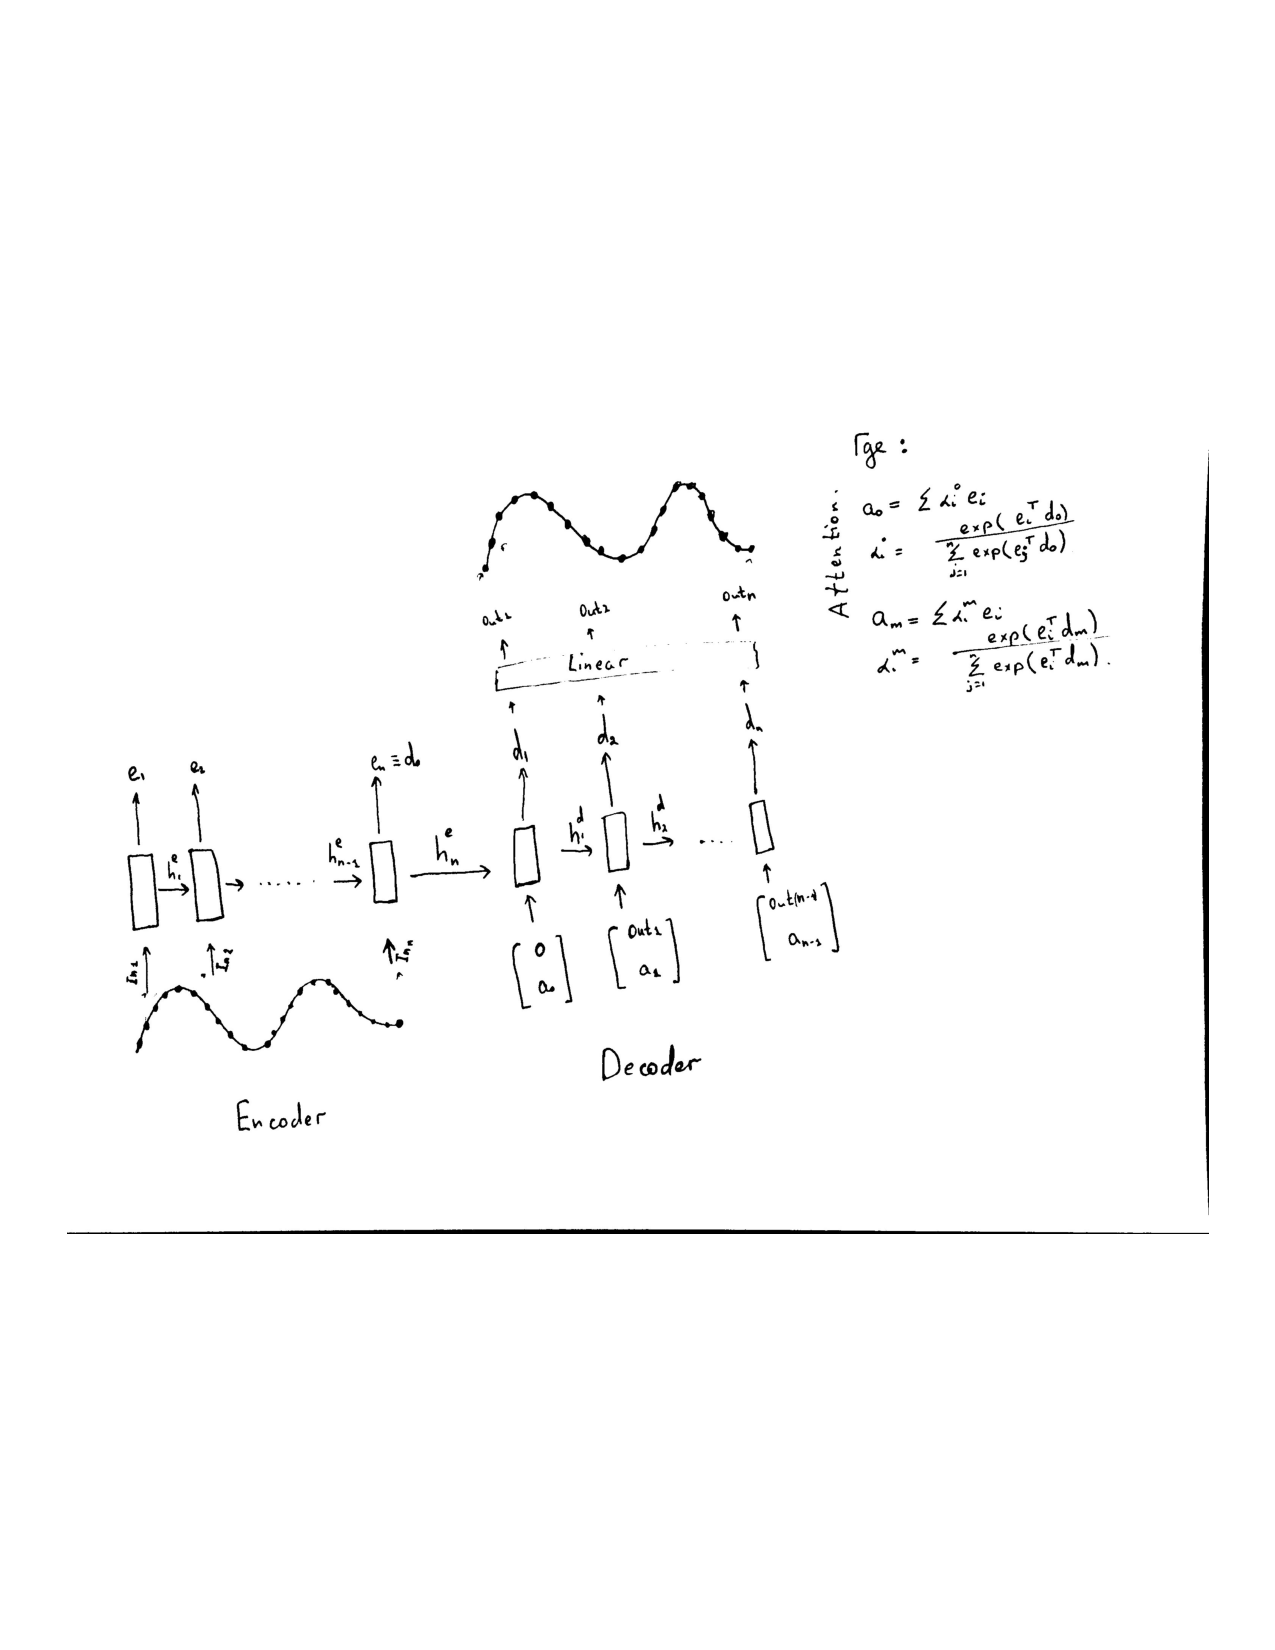
\includegraphics[width=0.5\textwidth]{figures/img1.pdf}\label{fig1}}
\subfloat[Описаниие предполагаемых результатов]{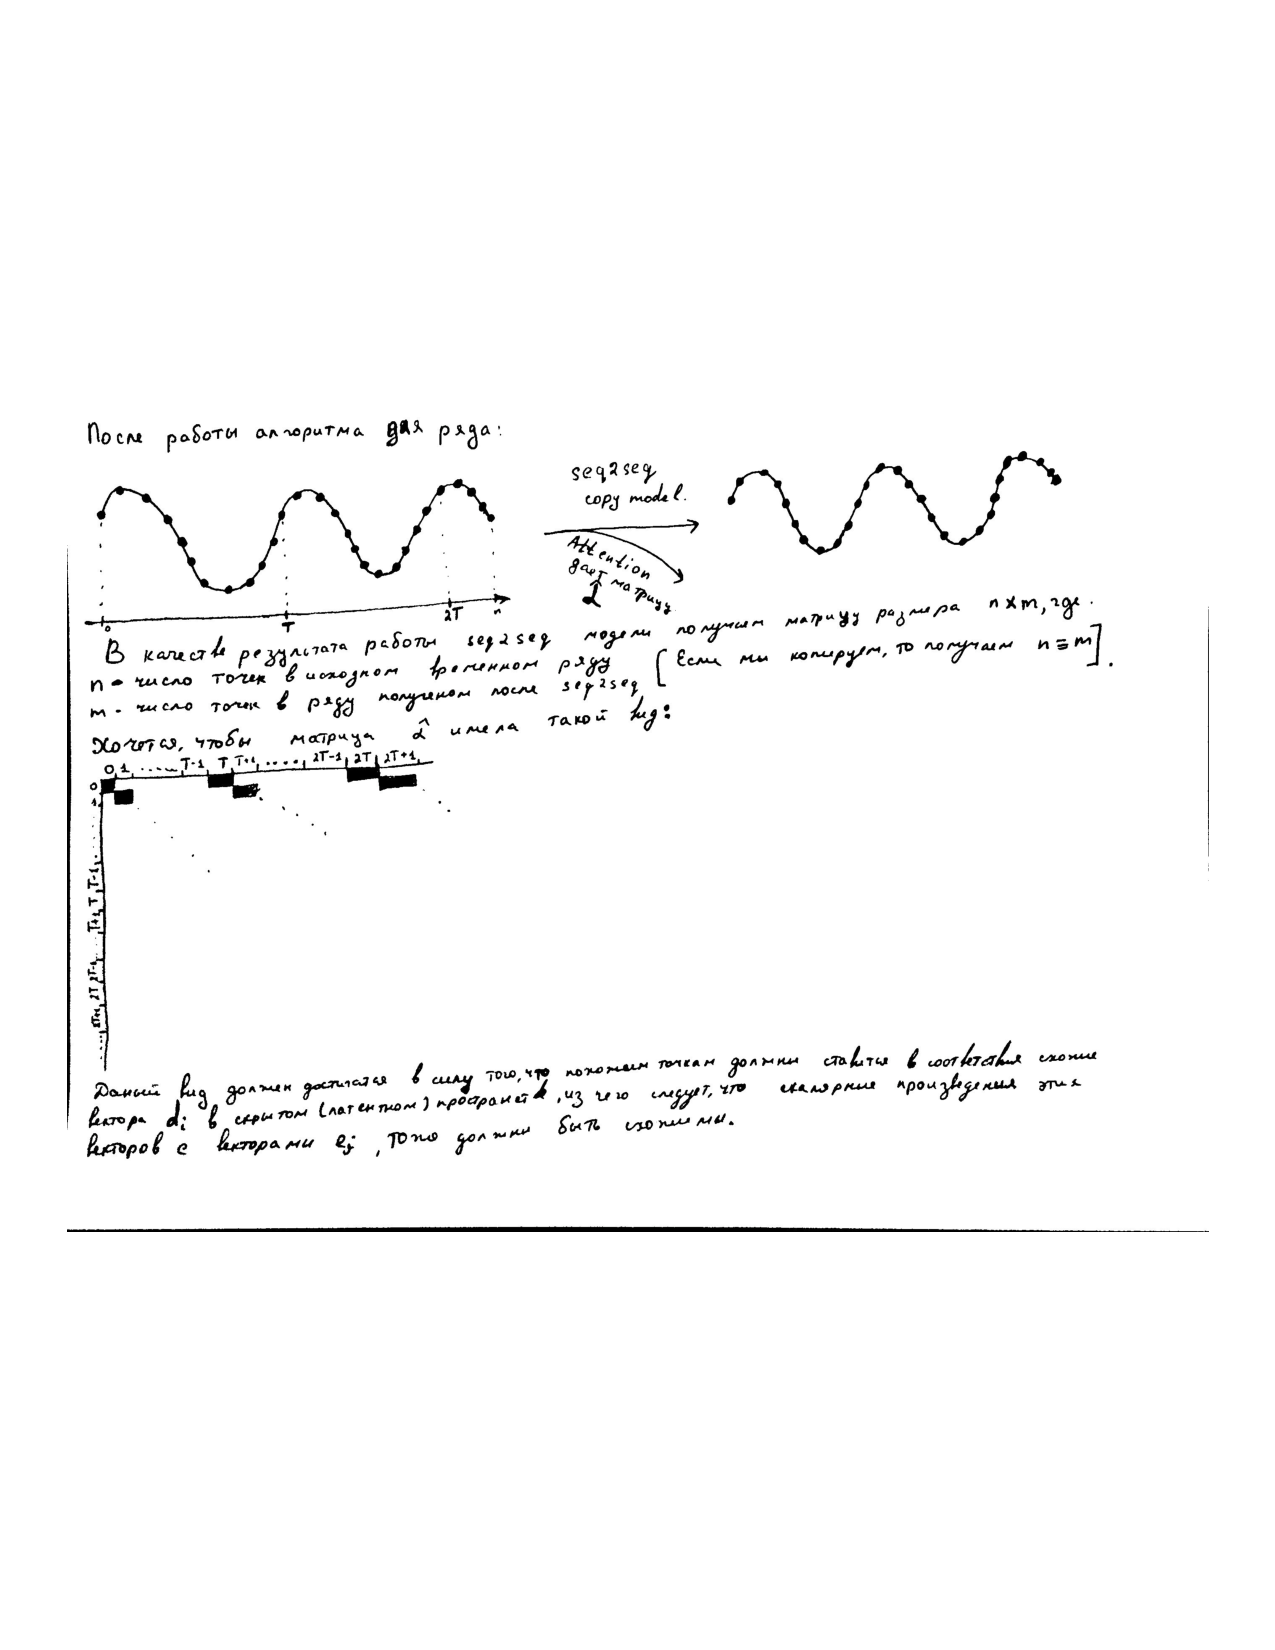
\includegraphics[width=0.5\textwidth]{figures/img2.pdf}\label{fig2}}
\caption{Основные сведения об seq2seq + Attention}
\end{figure}

Используем LSTM с простейшим Attention без дополнительных параметров. Пример, принцепа работы seq2seq c Attention показан на рис.~\ref{fig1}.

\section{Предположения}
Введя предположения о том, что скрытые вектора LSTM имеет похожие вектора для похожих кусков временного ряда можно предположить, что матрица Attention будет иметь вид показан на рис.~\ref{fig2}. Под матрицей Attention подрозумевается матрица размера $n\times m$, где $n, m$ --- длины входного и выходного сигналов соответственно, в ячейках которой показан уровень схожести (либо можно сказать уровень зависимости) между куском временного ряда на выходе и куском временного ряда на входе.

\section{Проблемы}
Предлагается использовать seq2seq, который просто копирует временной ряд. В этом методе есть ряд вопросов.
\begin{itemize}
    \item Первый косяк состоит в том, что если мы учим копировать временной ряд, и берем слишком сложный Attention с большим количеством параметров, то он начинает переобучатся, и в итоге получается матрица Attention диагональной. Это следует из того, что модель начинает просто учить друг за другом числа. Поэтому предлагается использовать просто скалярное произведение векторов (самую простую модель Attention, Dot метрика из~\ref{tab1}).
    
    \item Даже если взять простую модель Attention, все равно можно получить диагональную матрицу Attention, если мы просто будем копировать временной ряд, поэтому предлагается не просто учить все ряды из обучающего множества рядов, а на вход Encoder'а давать некоторый кусок (например из 100 сигналов ряда дать только первые 20 сигналов), и сравнивать как Decoder восстановит весь сигнал. Данный дополнительный финт немного улучшает качество.
    
    \item Второй вопрос состоит в том, что нужно придумать на каких данных учить данную модель (нужно подумать над тем какие сигналы давать на вход для копирования). Этот вопрос возникает в синтетических данных, но и в реальных данных. Я думаю, что можно модель учить не только на реальных данных, а и на синтетических, но для этого нужно придумать максимально правдоподобный сигнал акселерометра.
    
\end{itemize}

\begin{table}[h!]
\begin{center}
\caption{Описание разных Attention}
\label{tab1}
\begin{tabular}{|c|c|}
\hline
	Type & formula\\
	\hline
	Additive& $score_{i,j}~=~\textbf{w}_o\tanh\left(\textbf{W}_e\textbf{e}_i+\textbf{W}_d\textbf{d}_j\right)$\\
	\hline
	Dot& $score_{i,j}~=~\textbf{e}_i^{\mathsf{T}}\textbf{d}_j$\\
	\hline
	General& $score_{i,j}~=~\textbf{e}_i^{\mathsf{T}}\textbf{W}\textbf{d}_j$\\
\hline
\end{tabular}

\end{center}
\end{table}

\section{Эксперимент}
\subsection{Эксперимент с простыми периодическими структурами}

\begin{figure}[h!t]\center
\subfloat[$sin(x)$]{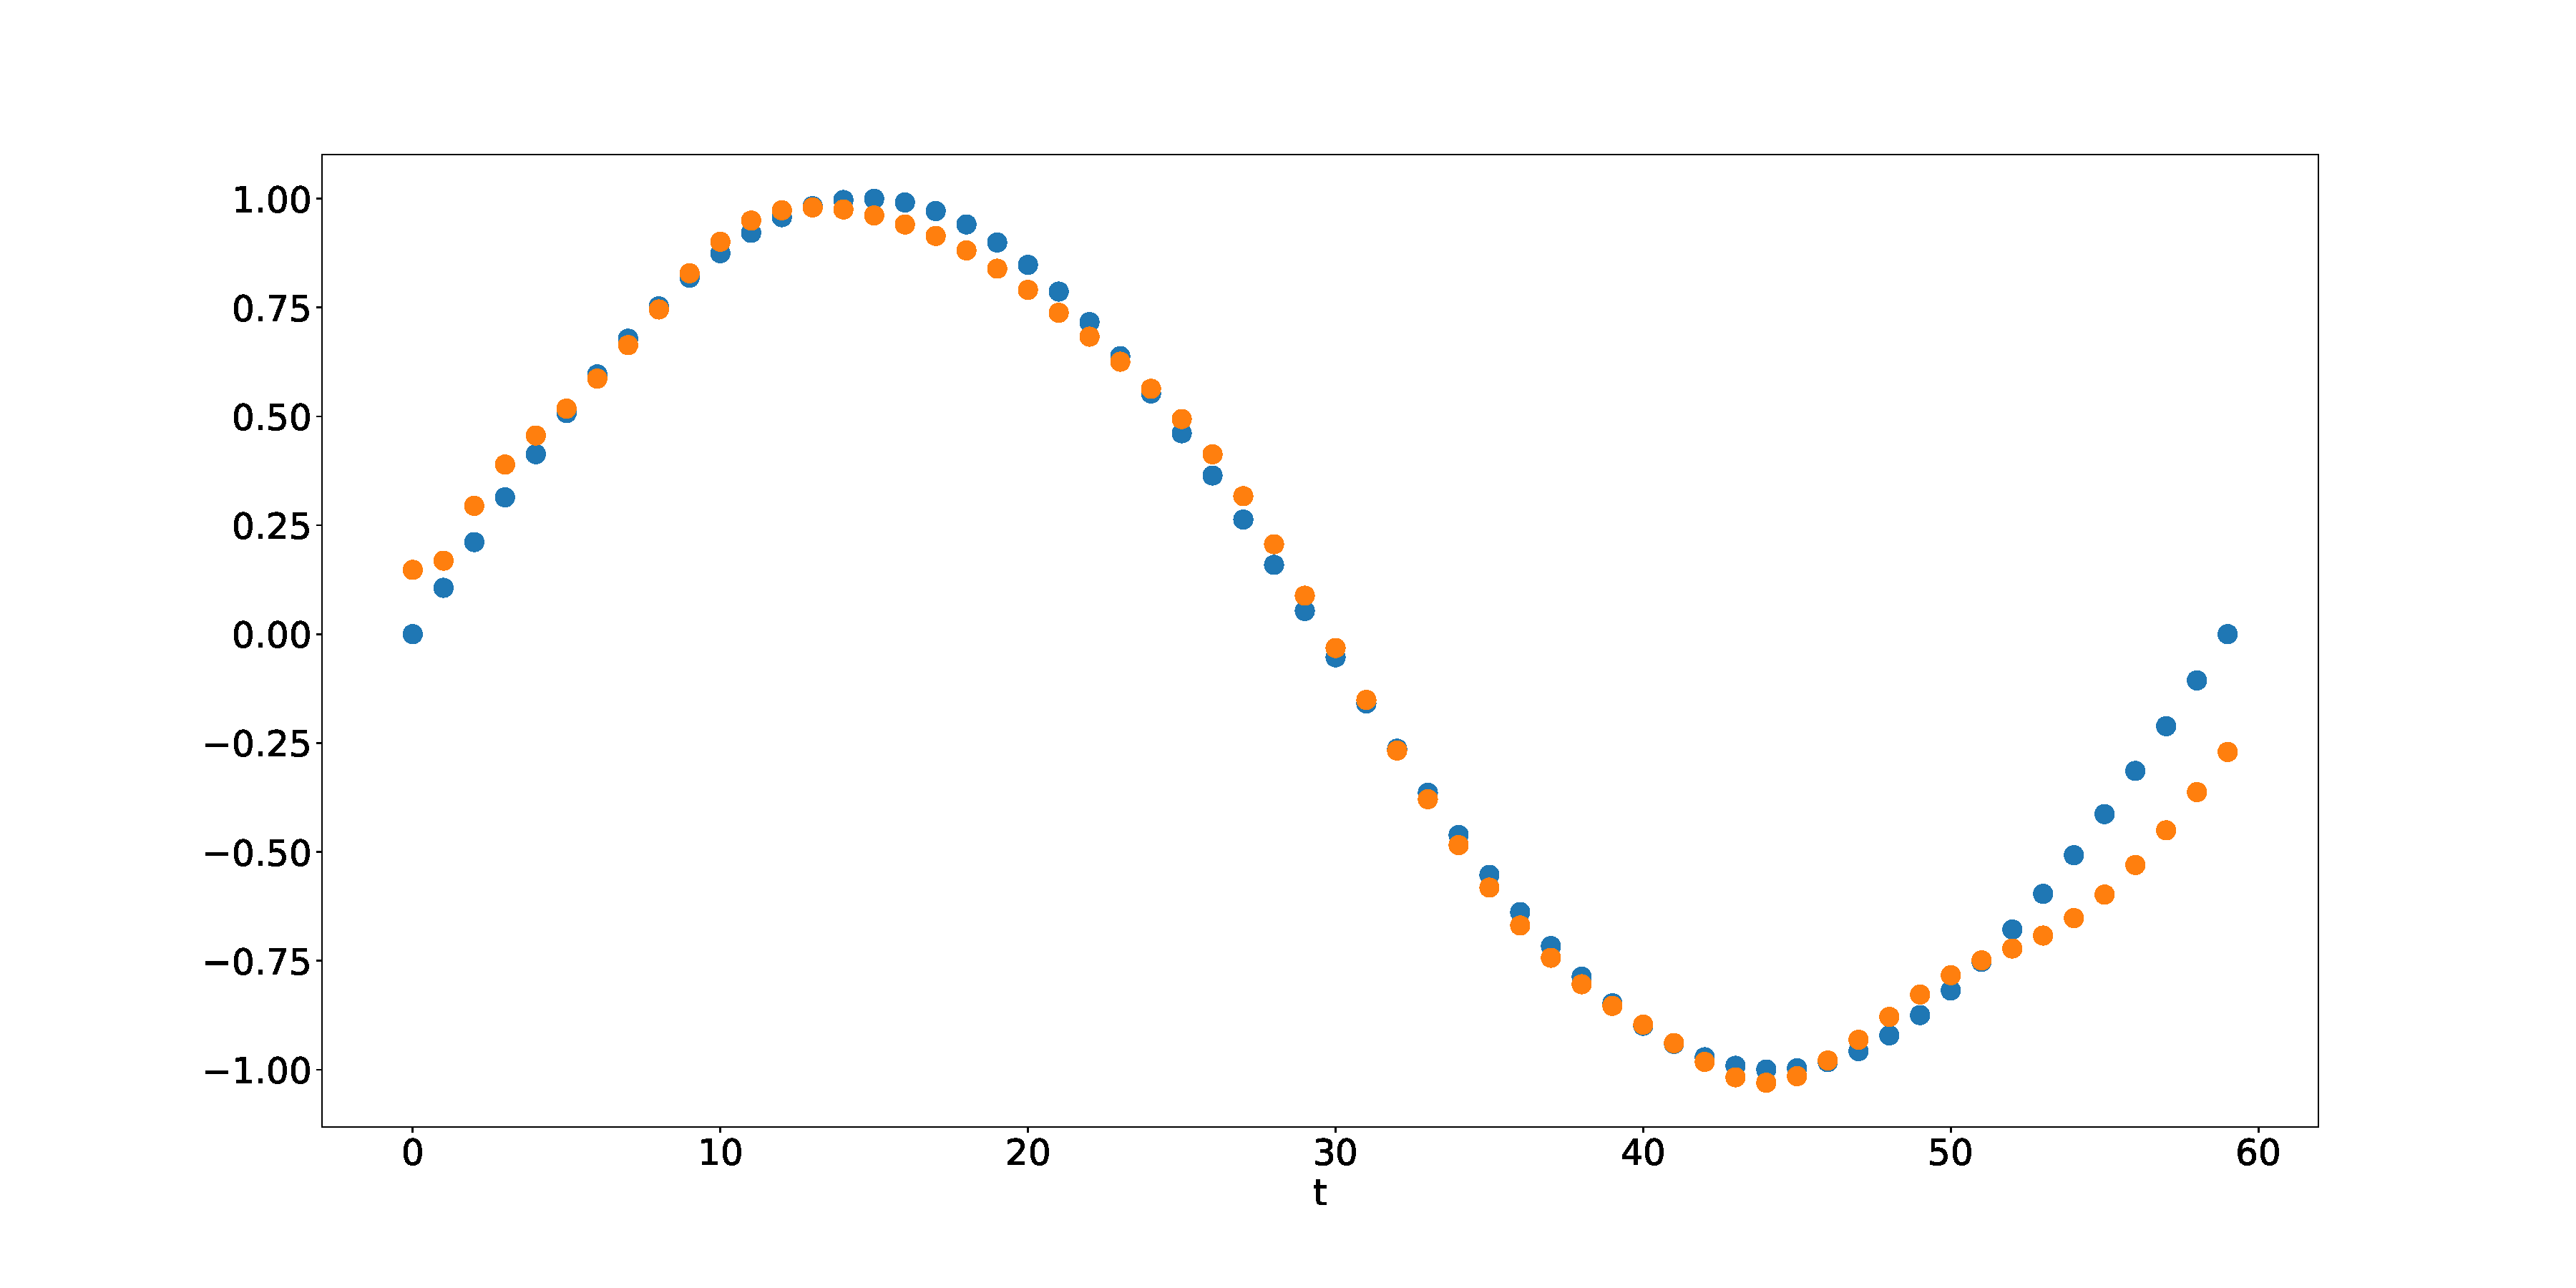
\includegraphics[width=0.5\textwidth]{figures/TimeSeries1.pdf}}
\subfloat[$sin(x)$]{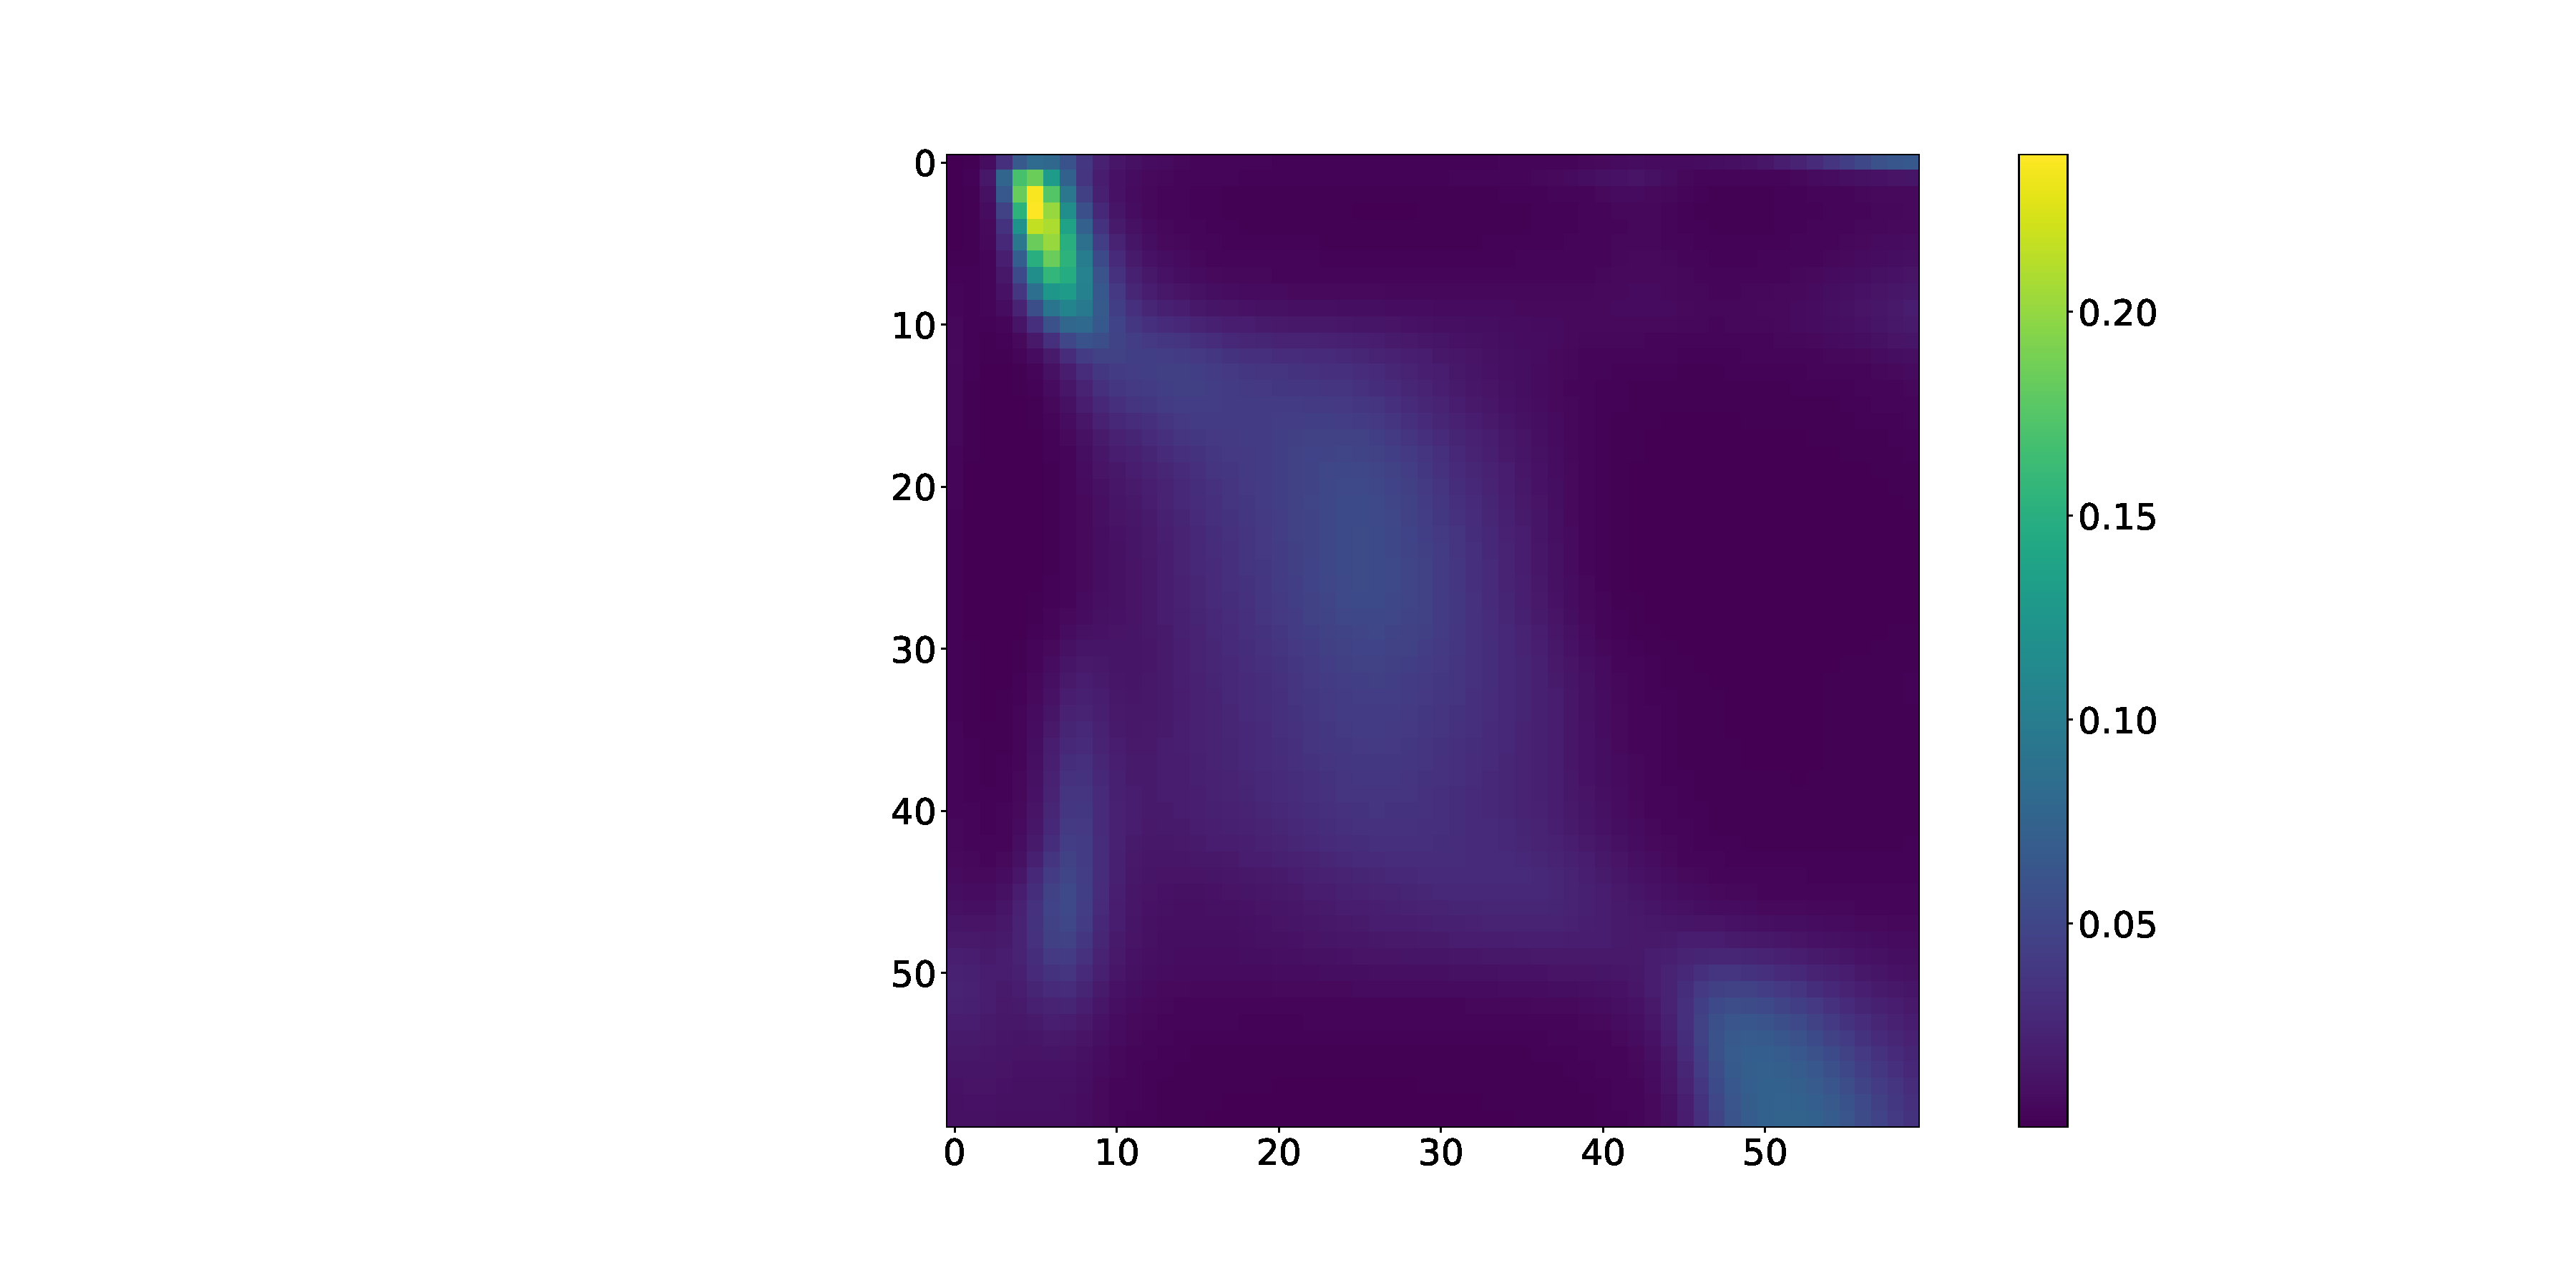
\includegraphics[width=0.5\textwidth]{figures/Attention1.pdf}}\\
\subfloat[$sin(2x)$]{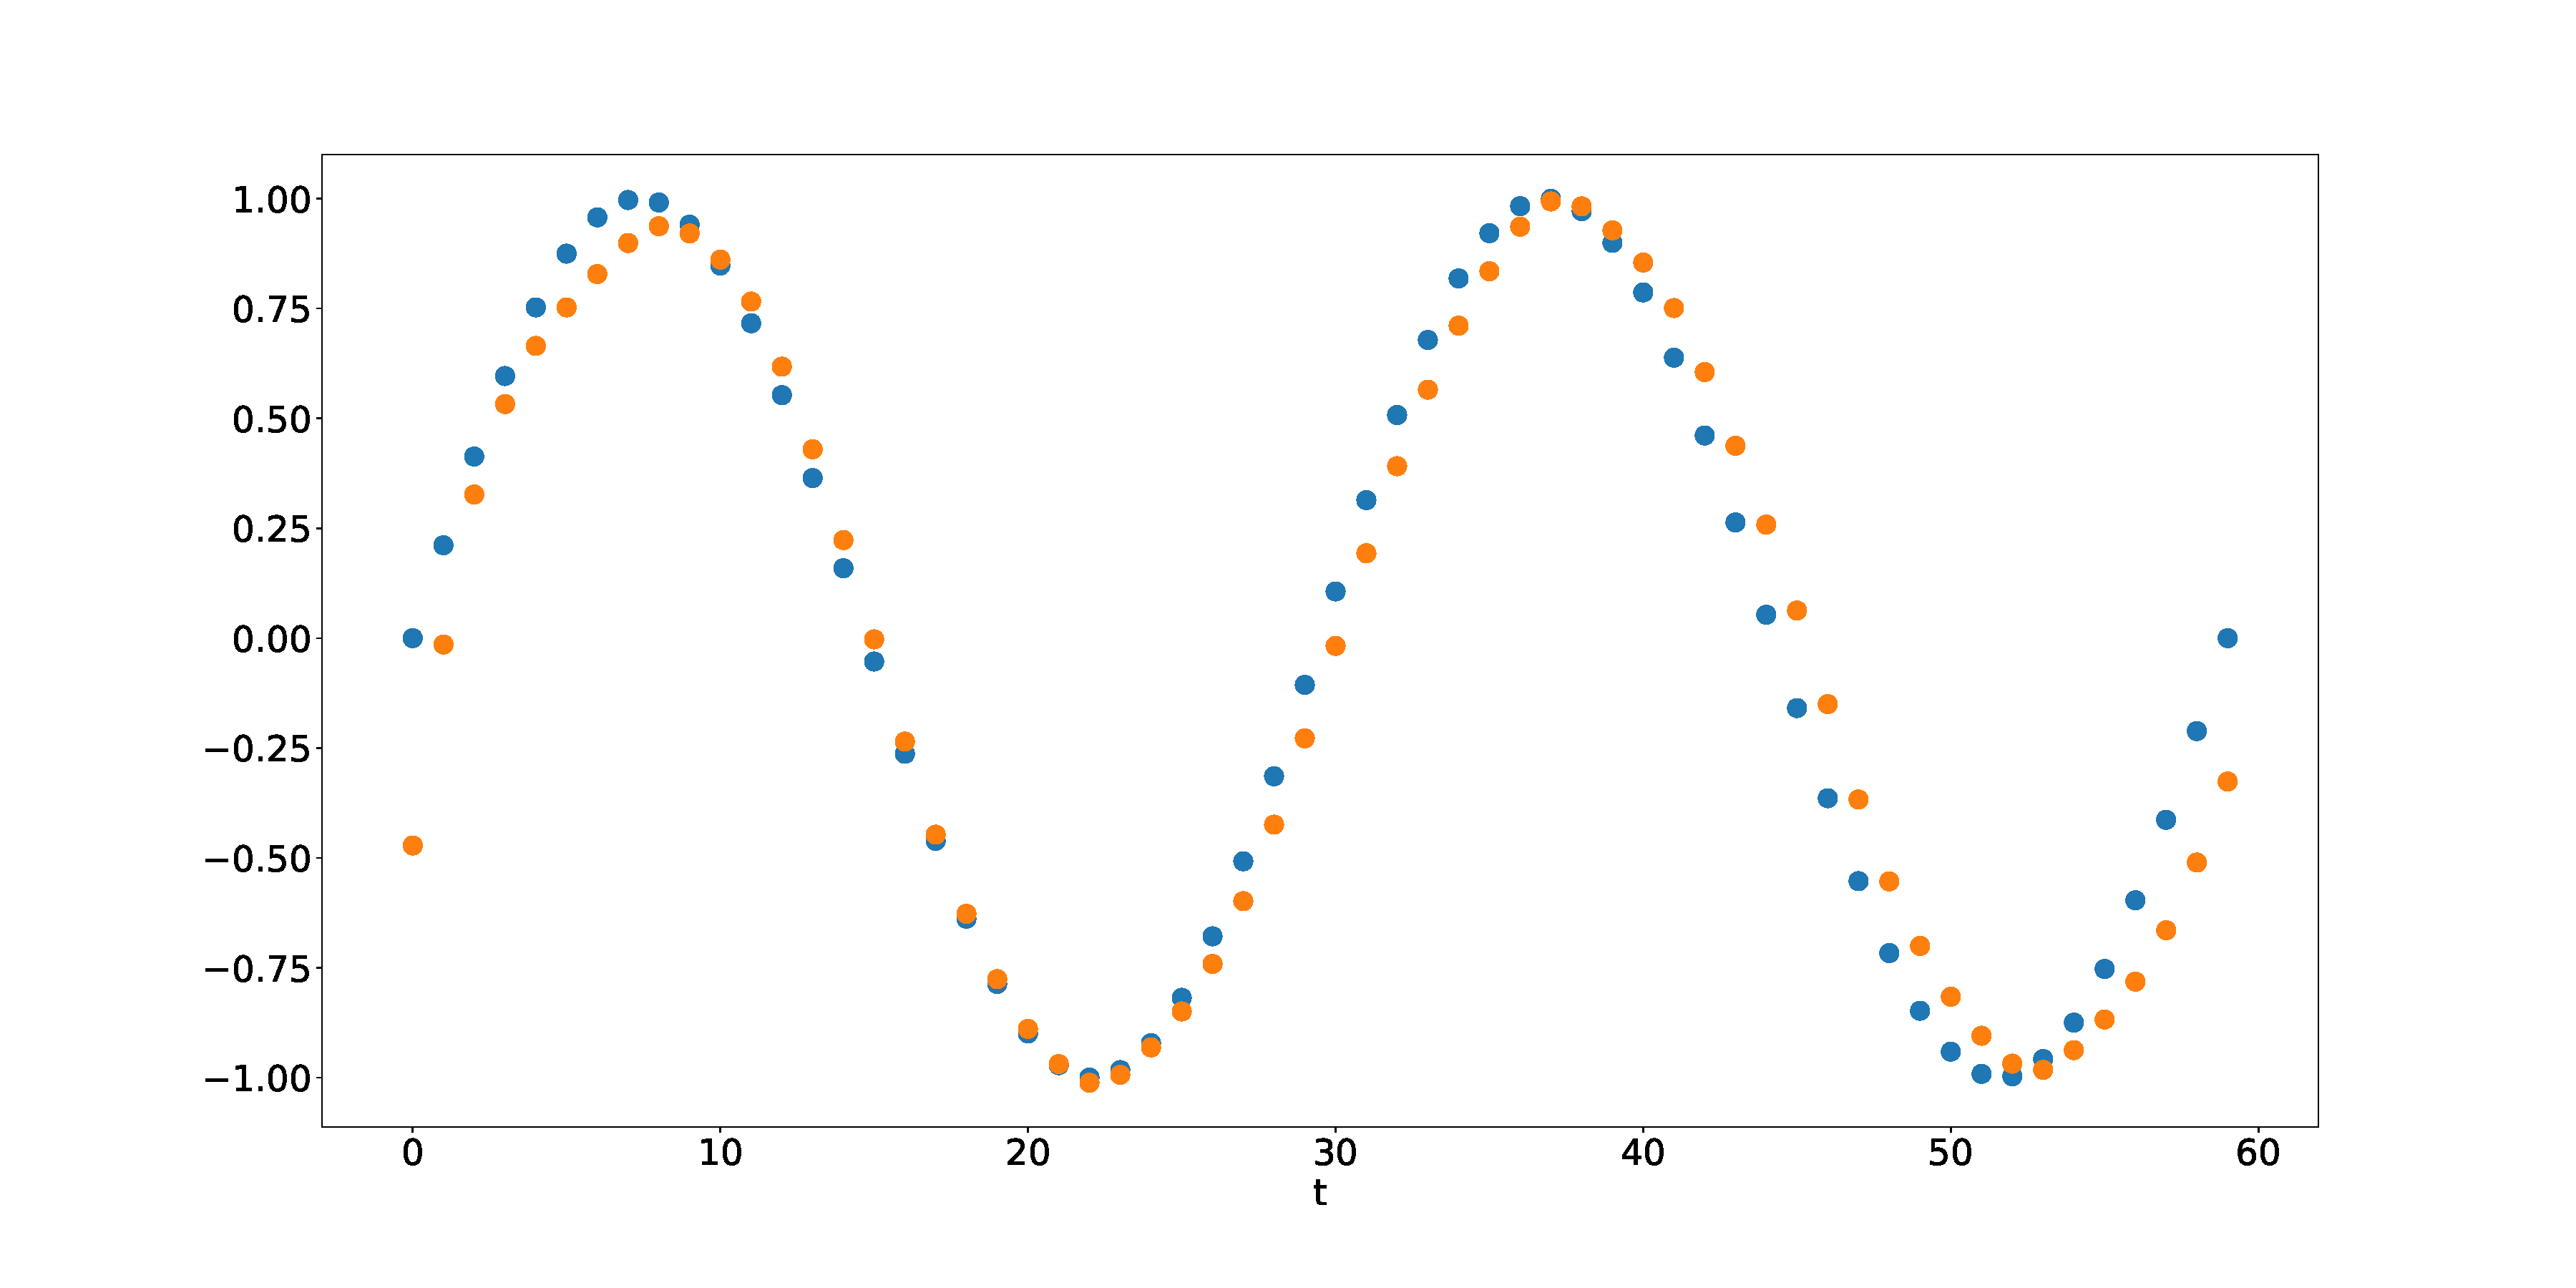
\includegraphics[width=0.5\textwidth]{figures/TimeSeries2.pdf}}
\subfloat[$sin(2x)$]{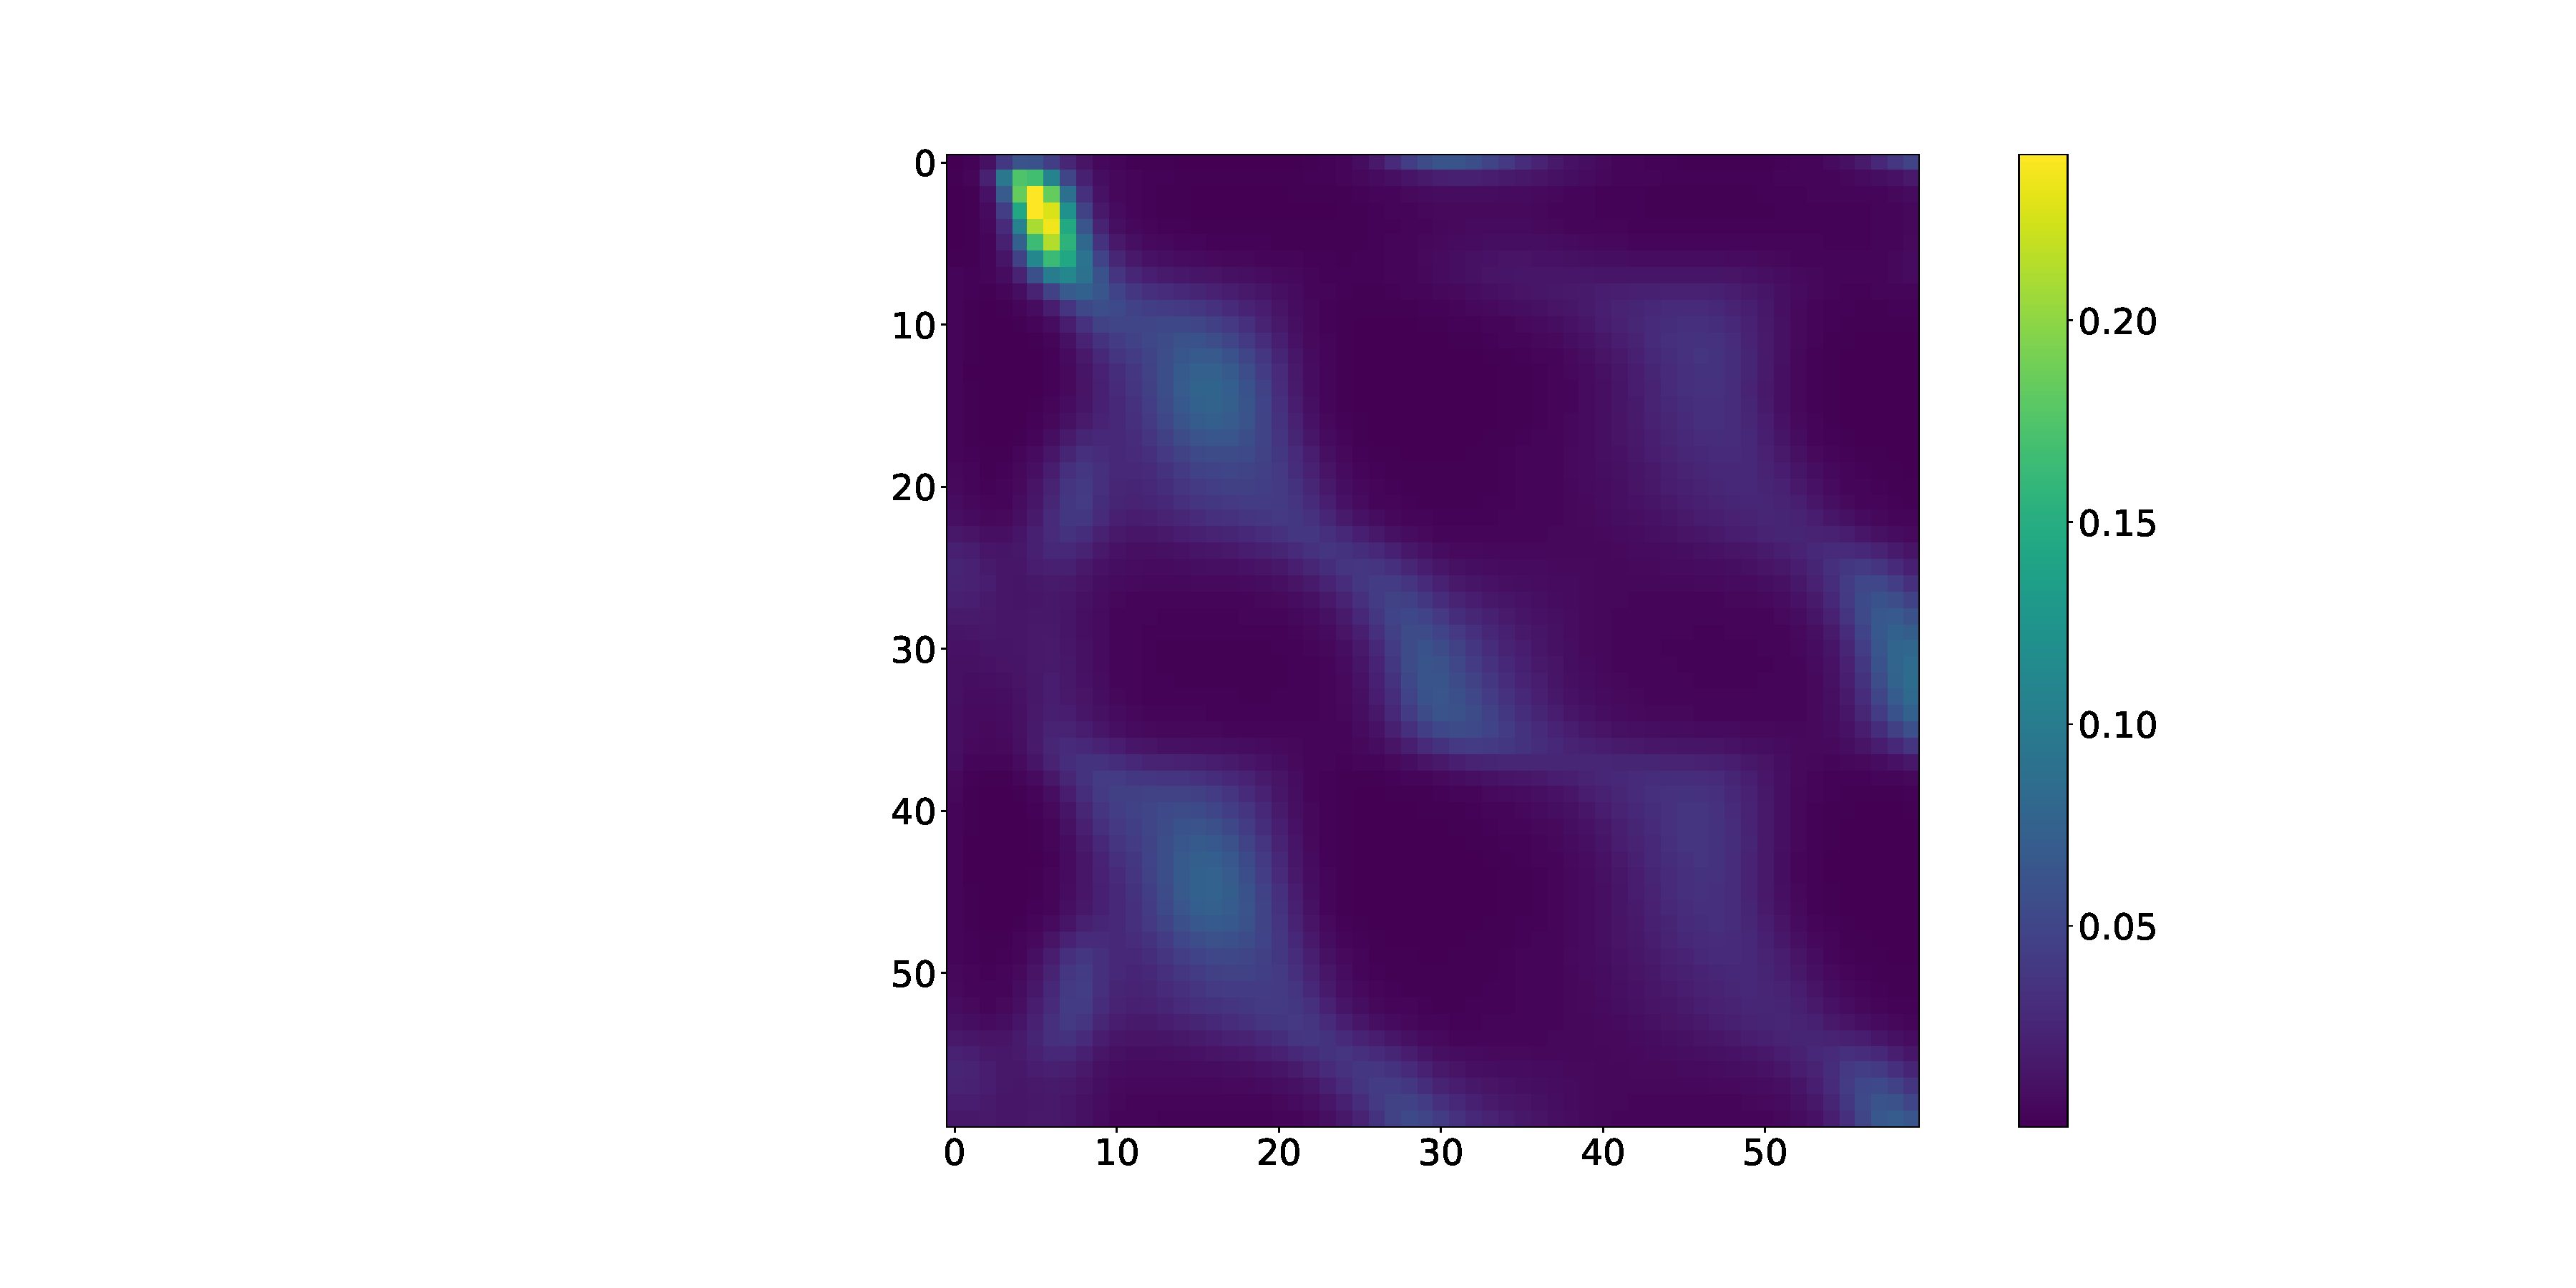
\includegraphics[width=0.5\textwidth]{figures/Attention2.pdf}}\\
\subfloat[$sin(8x)$]{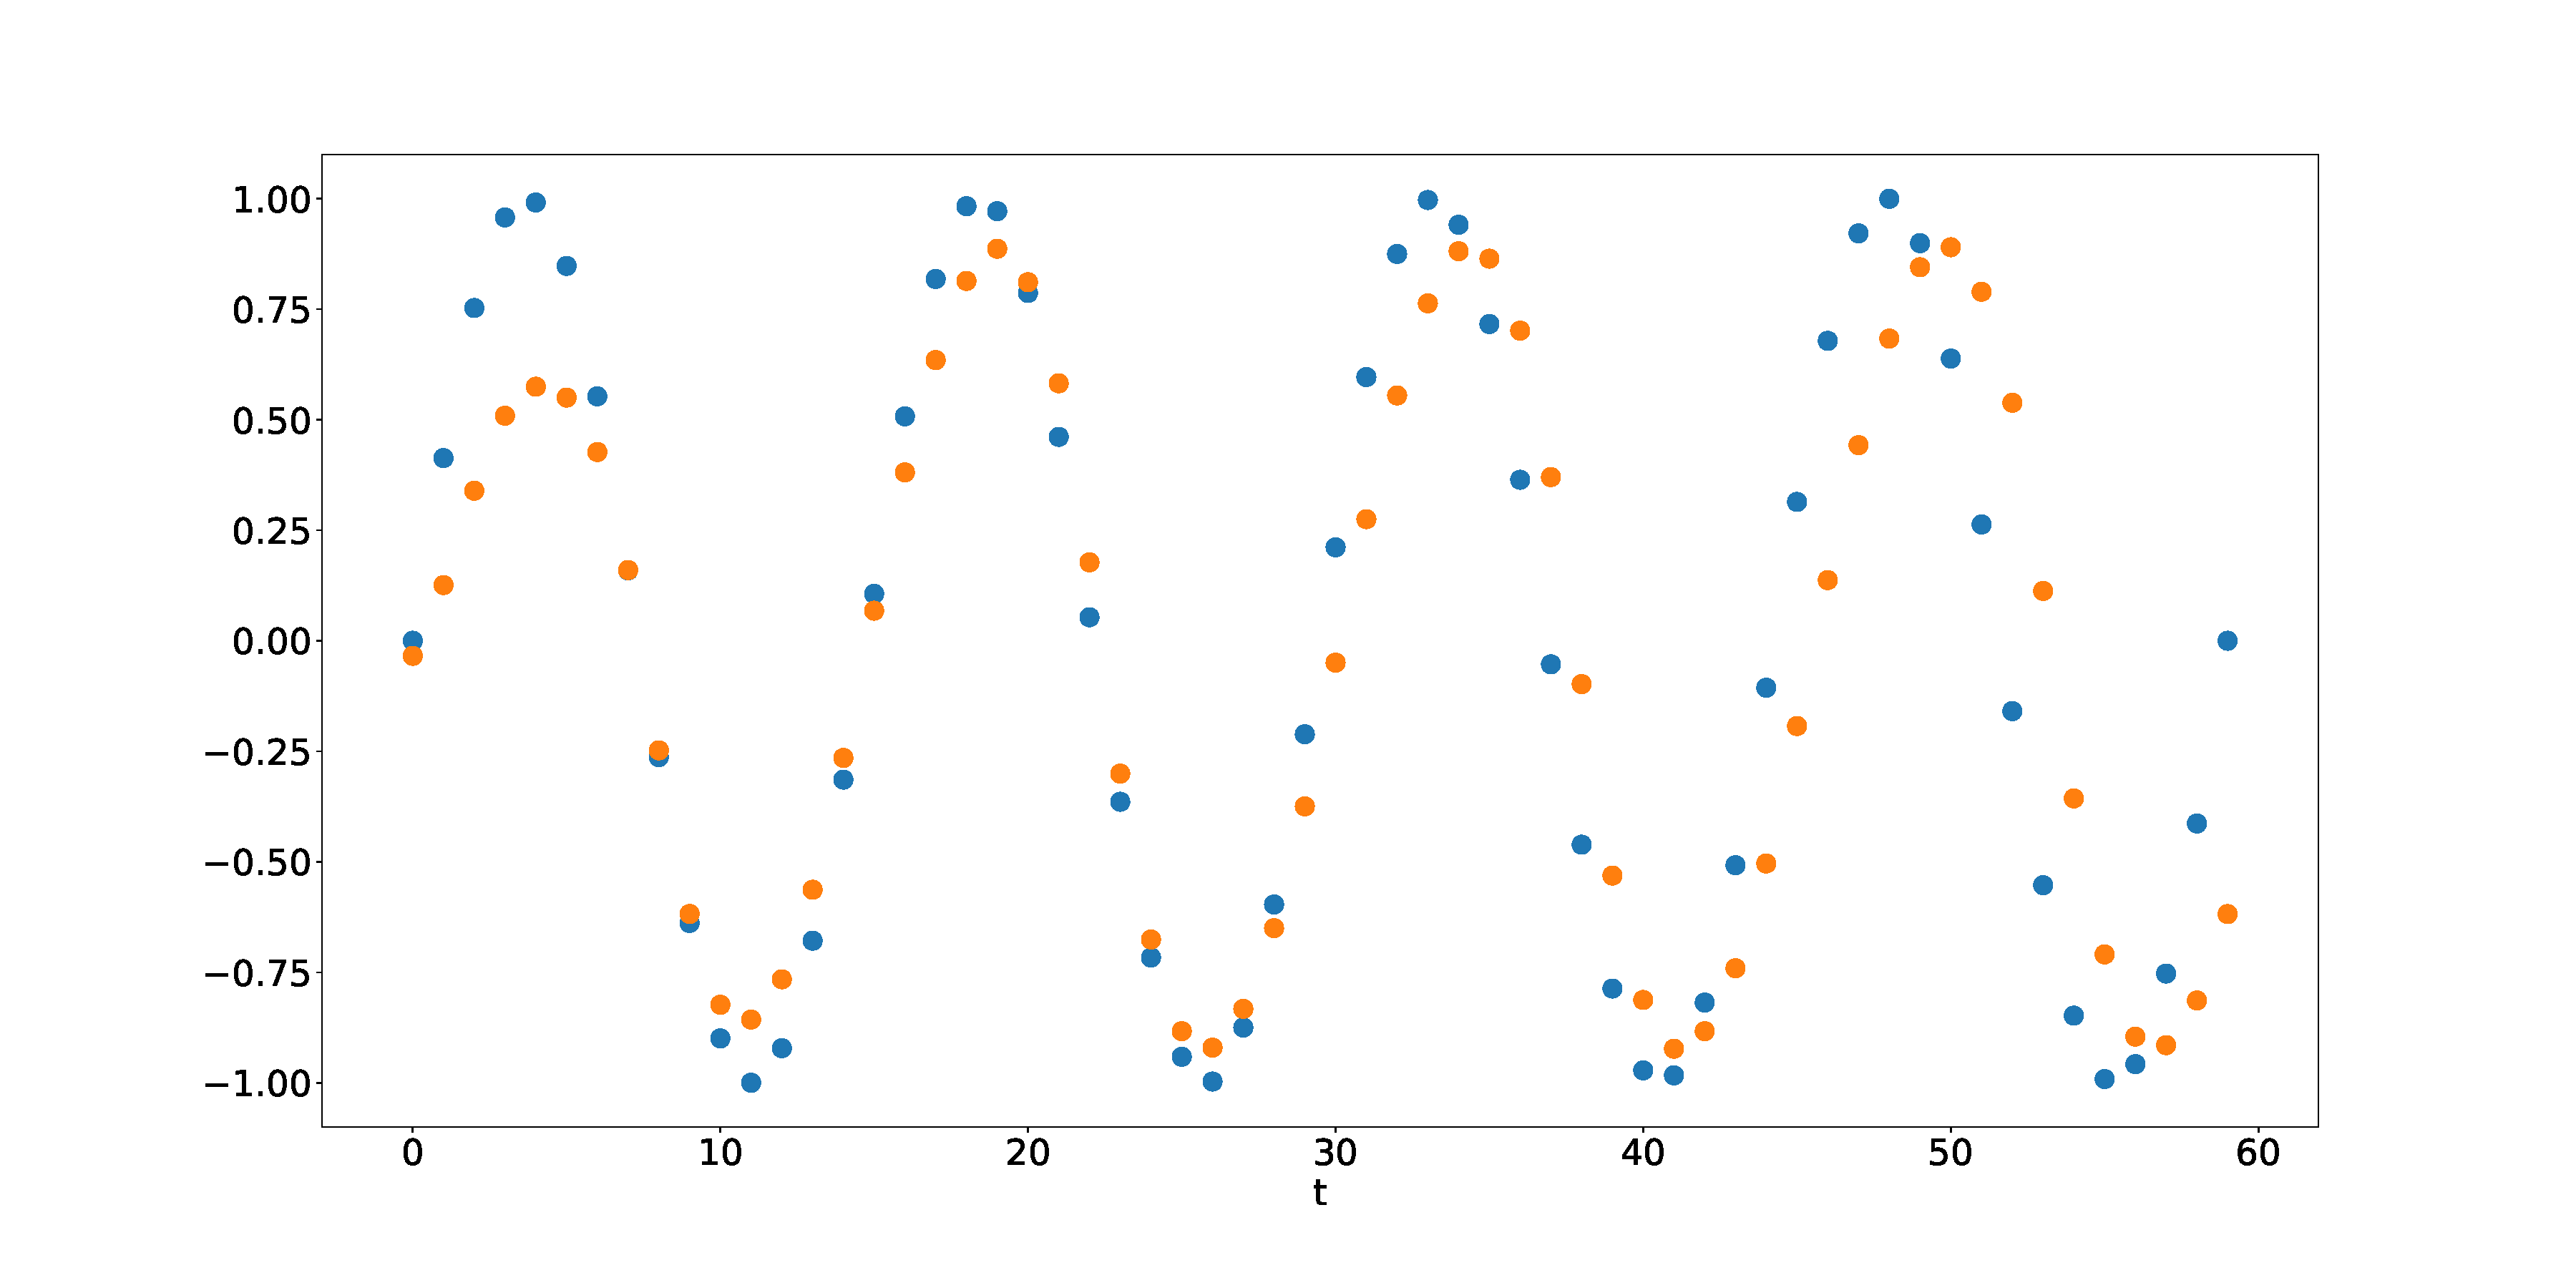
\includegraphics[width=0.5\textwidth]{figures/TimeSeries3.pdf}}
\subfloat[$sin(8x)$]{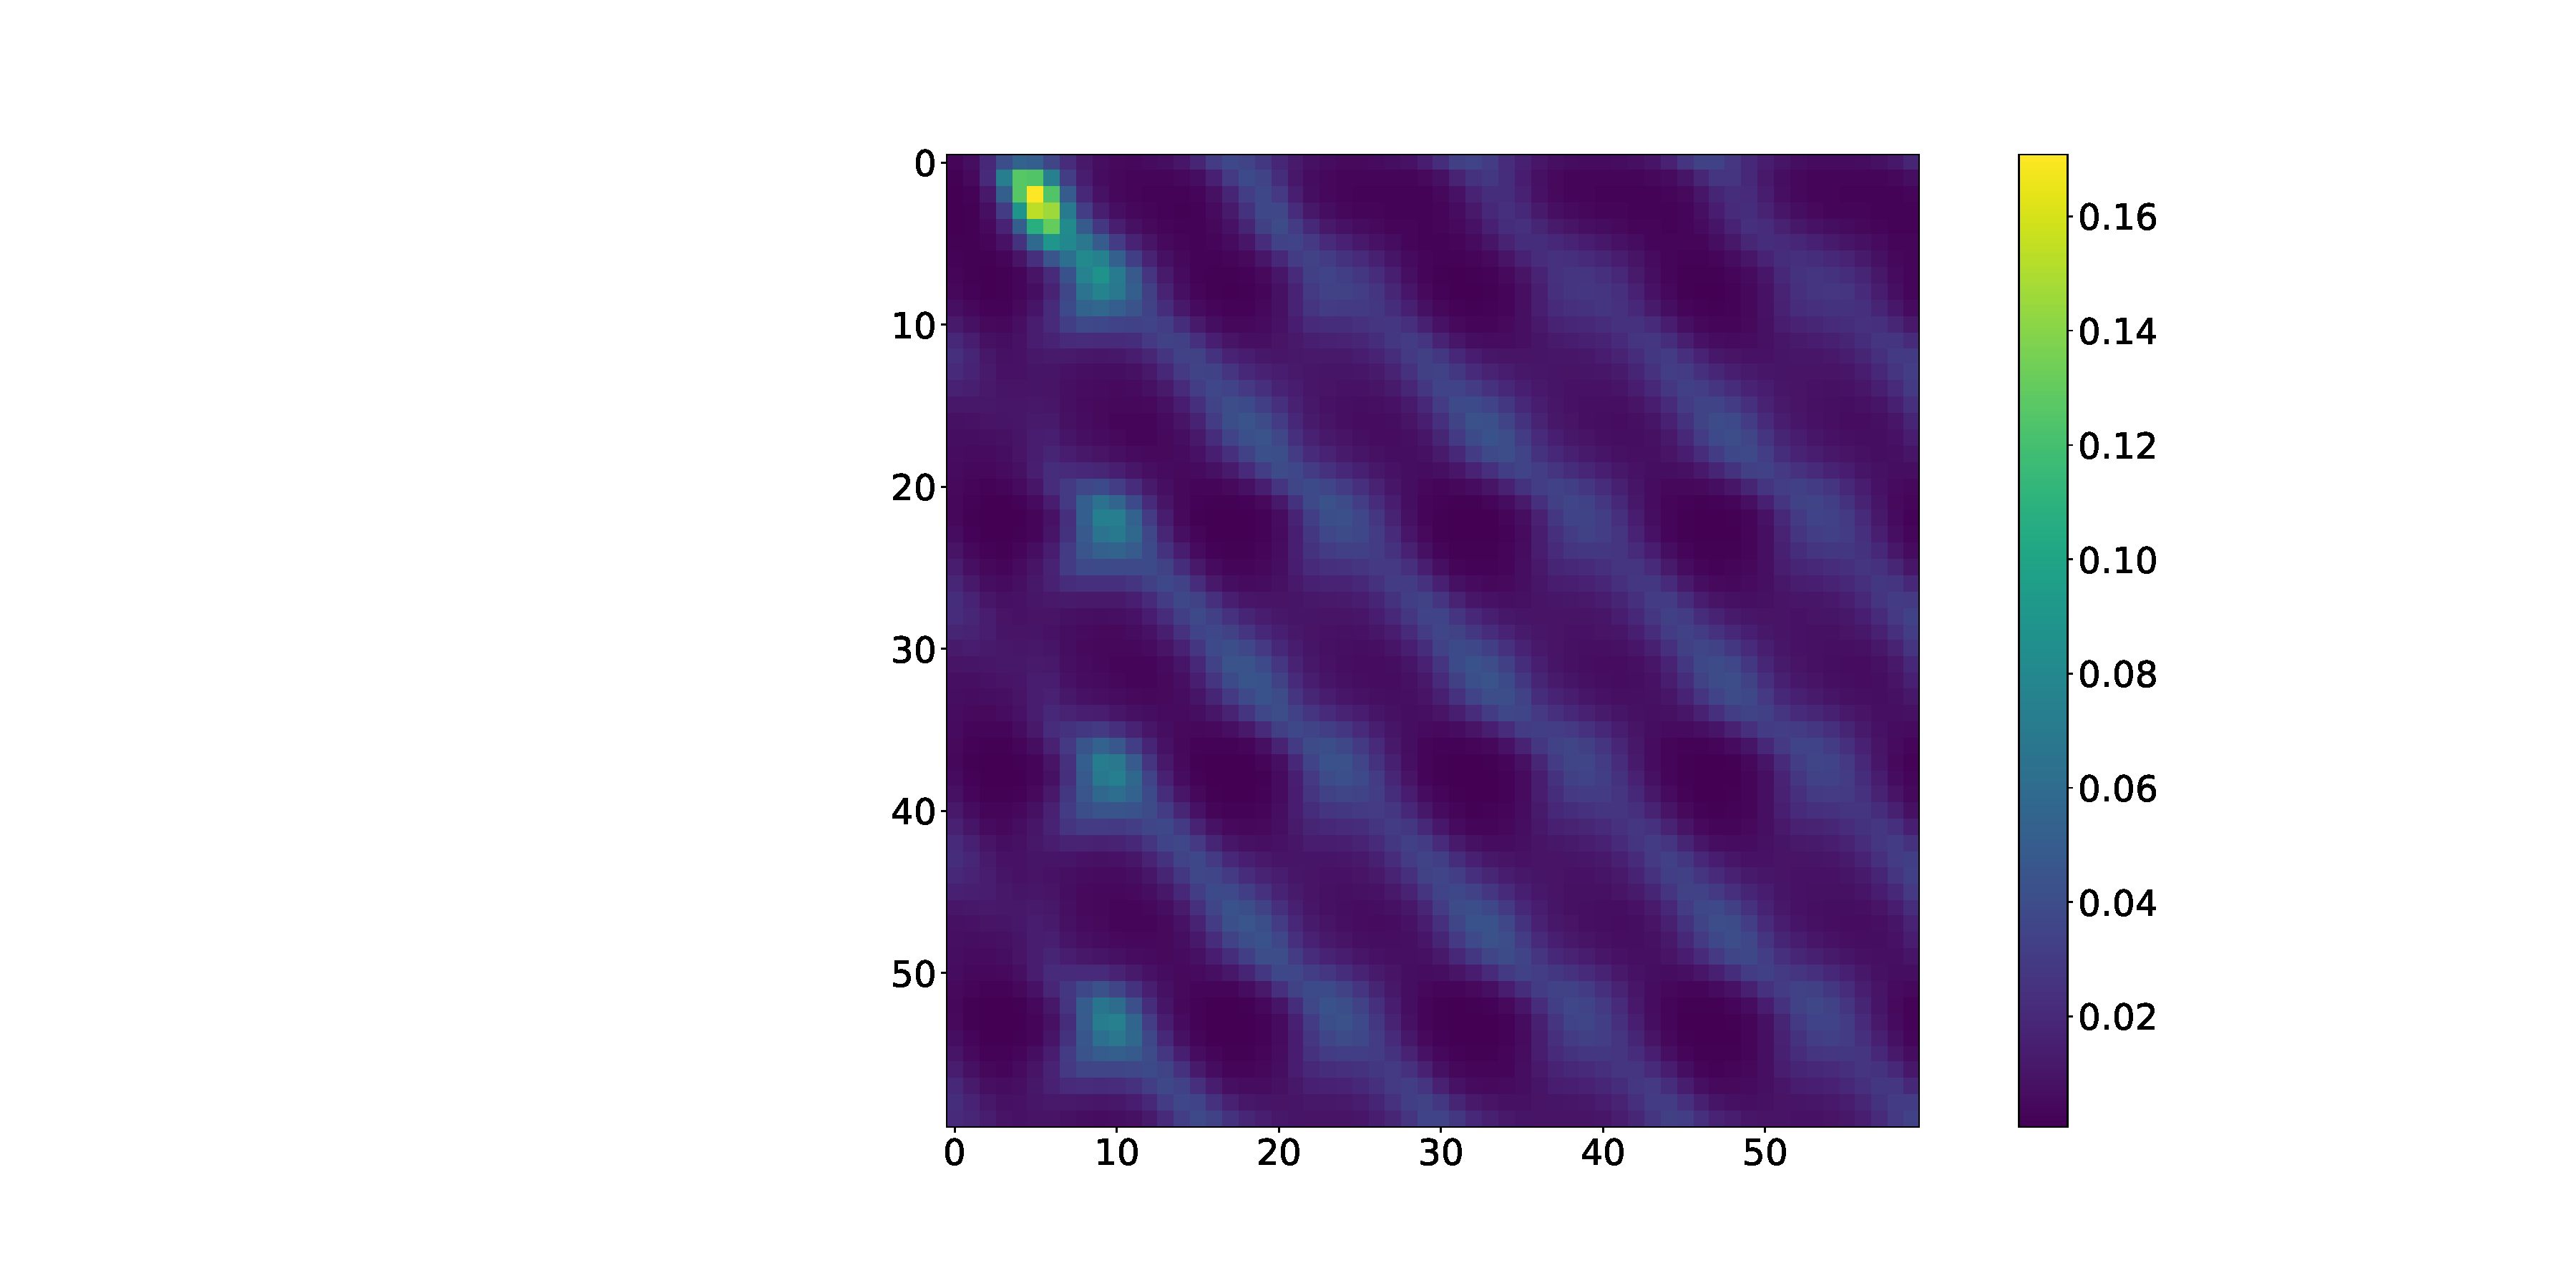
\includegraphics[width=0.5\textwidth]{figures/Attention3.pdf}}\\

\caption{Результаты для модели с рис.~\ref{fig1}}
\label{fig3}
\end{figure}



Пусть модель обучена на синусоидальных сигналах с произвольной частотой, произвольной амплитудой и произвольной начальной фазой. Как видно из результатов на рис.~\ref{fig3}, предположение о виде матрицы Attention подтверждается. На рис~\ref{fig3} показано как меняется вид матрицы Attention в зависимости от частоты синуса. Видно что количество диагоналей в матрице Attention соответствует частоте синусоидального сигнала.

В работе~\cite{cinar2018} показано, что для нахождения периодов во временном ряде нельзя использовать простой Attention. Был пердложен модифицированный Attention который виглядит в следующем виде:

$$e_{ij}=~=~\textbf{w}_o\tanh\left(\textbf{W}_e\left(\bm{\pi}_{i-j}\textbf{e}_i\right)+\textbf{W}_d\textbf{d}_j\right)\cdot \left[i-j \leq T\right], \eqno(1)$$
где $\bm{\pi}$ --- еще один обучаемый вектор параметров, который указывает на степень зависимости $i$-го и $j$-го элемента.
	
Мои эксперименты показали, что прирост качества в двух разных Attention не очень большой, поэтому можно использовать любой из них.


\subsection{Эксперимент с простыми переодическими структурами в случае размерности скрытого пространства $2$}


\begin{figure}[h!t]\center
\subfloat[]{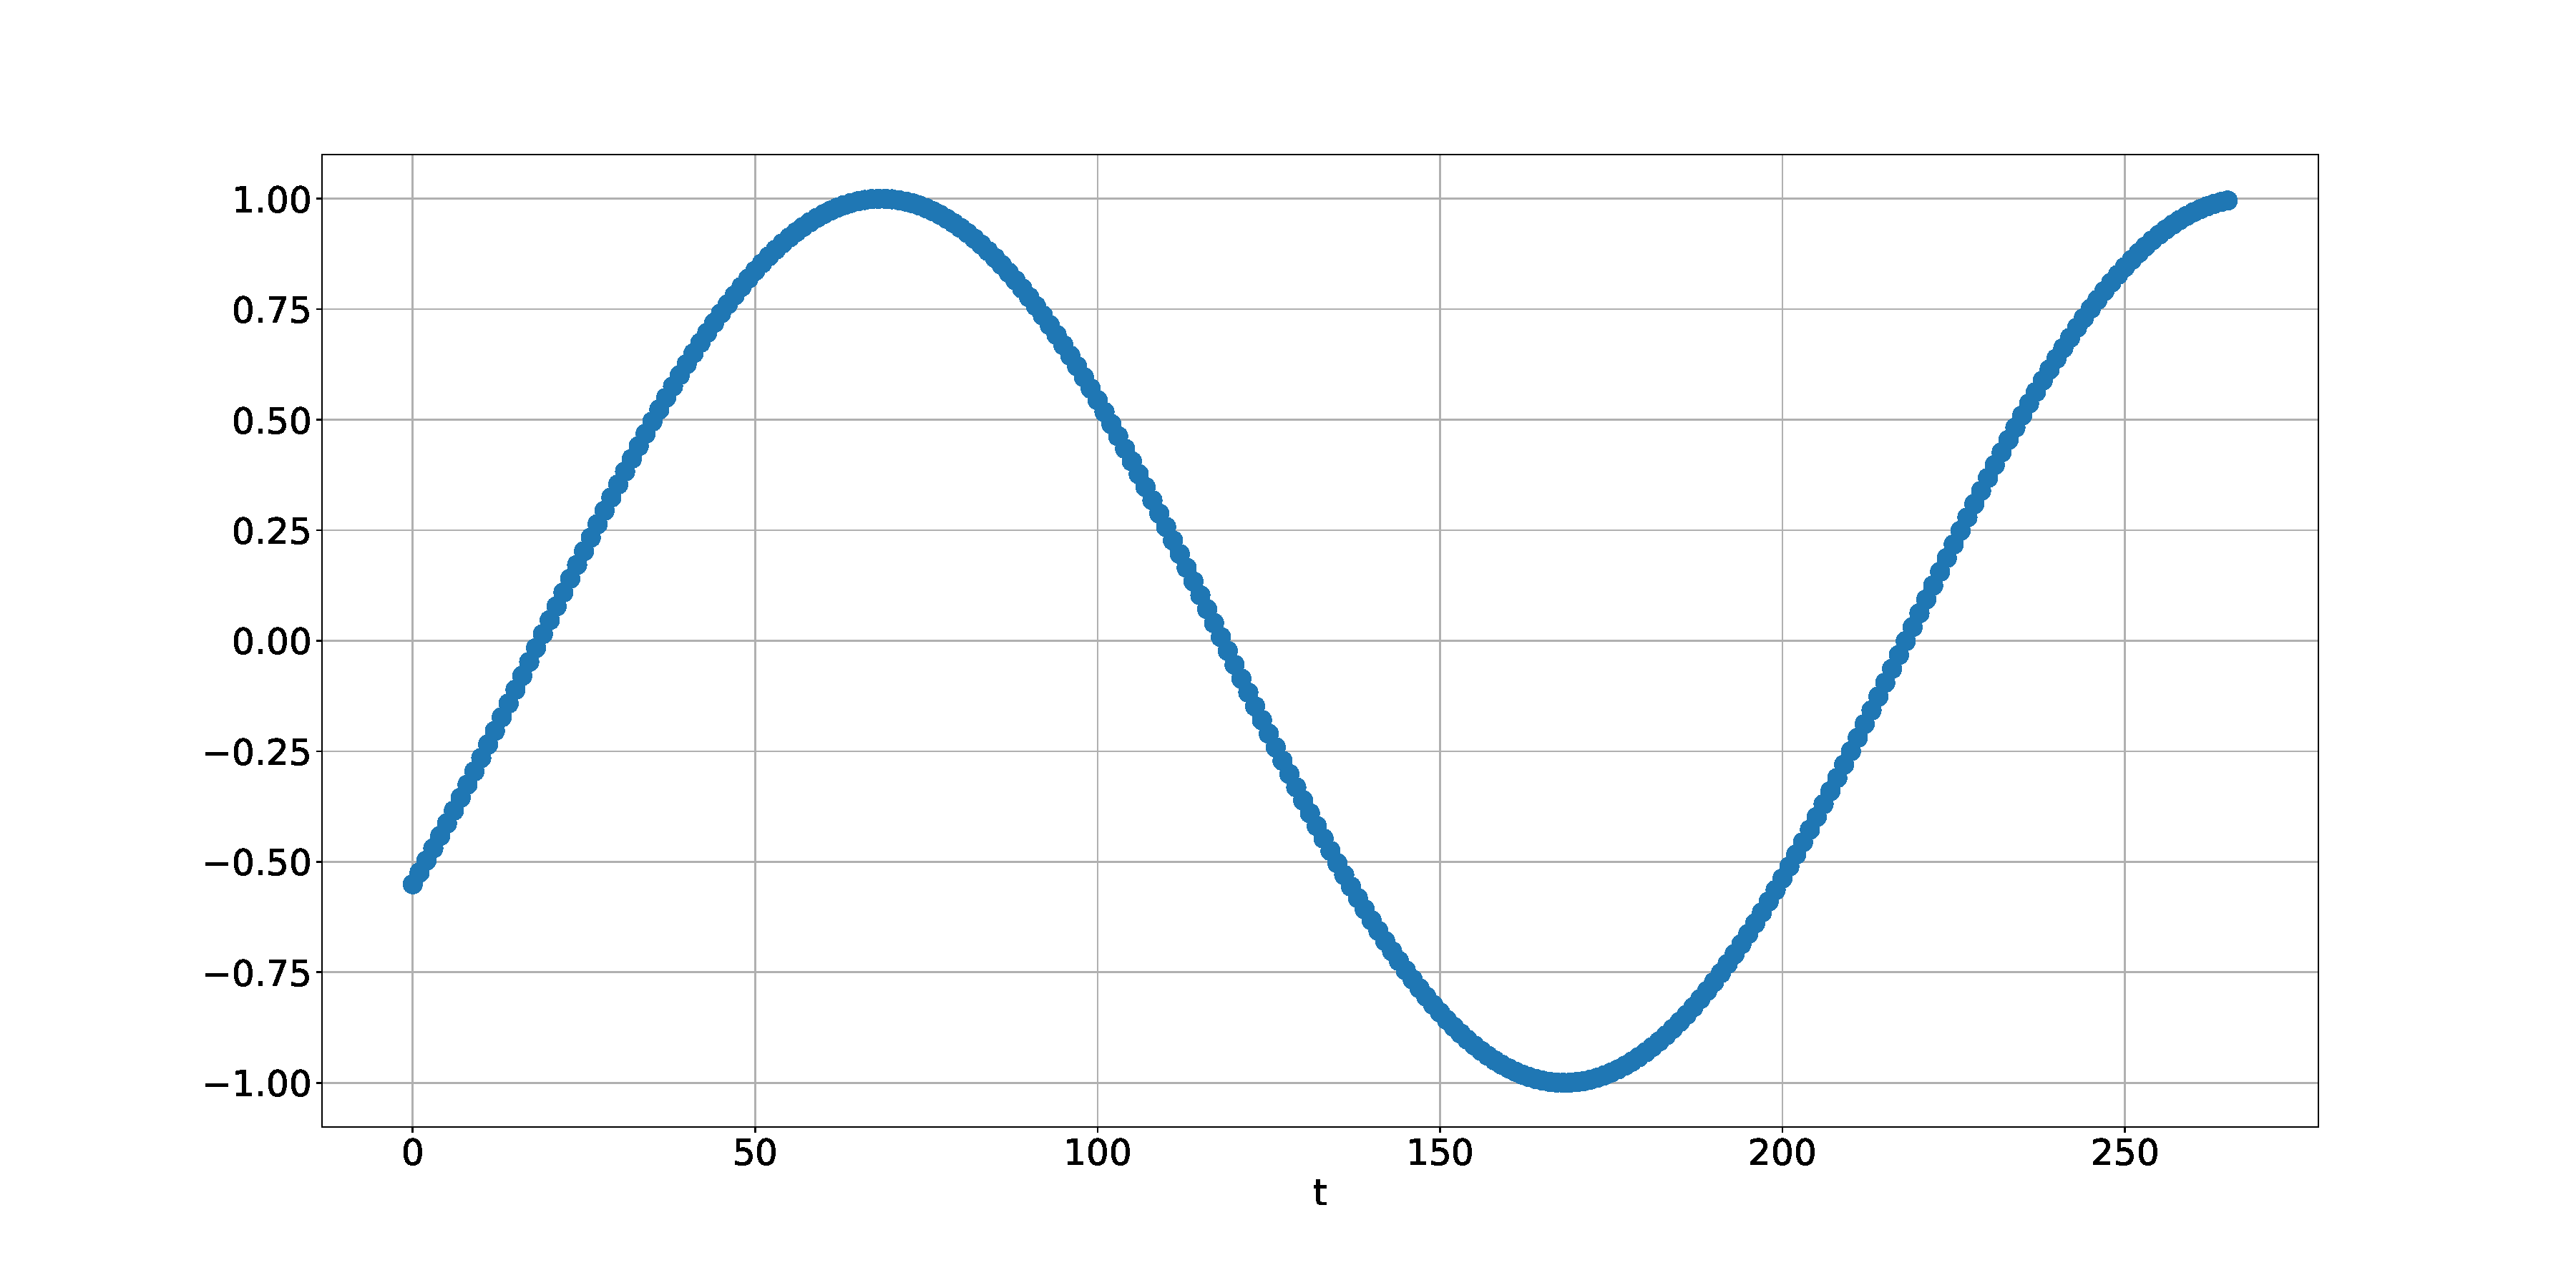
\includegraphics[width=0.5\textwidth]{figures/TimeSeries1_2dim.pdf}}
\subfloat[]{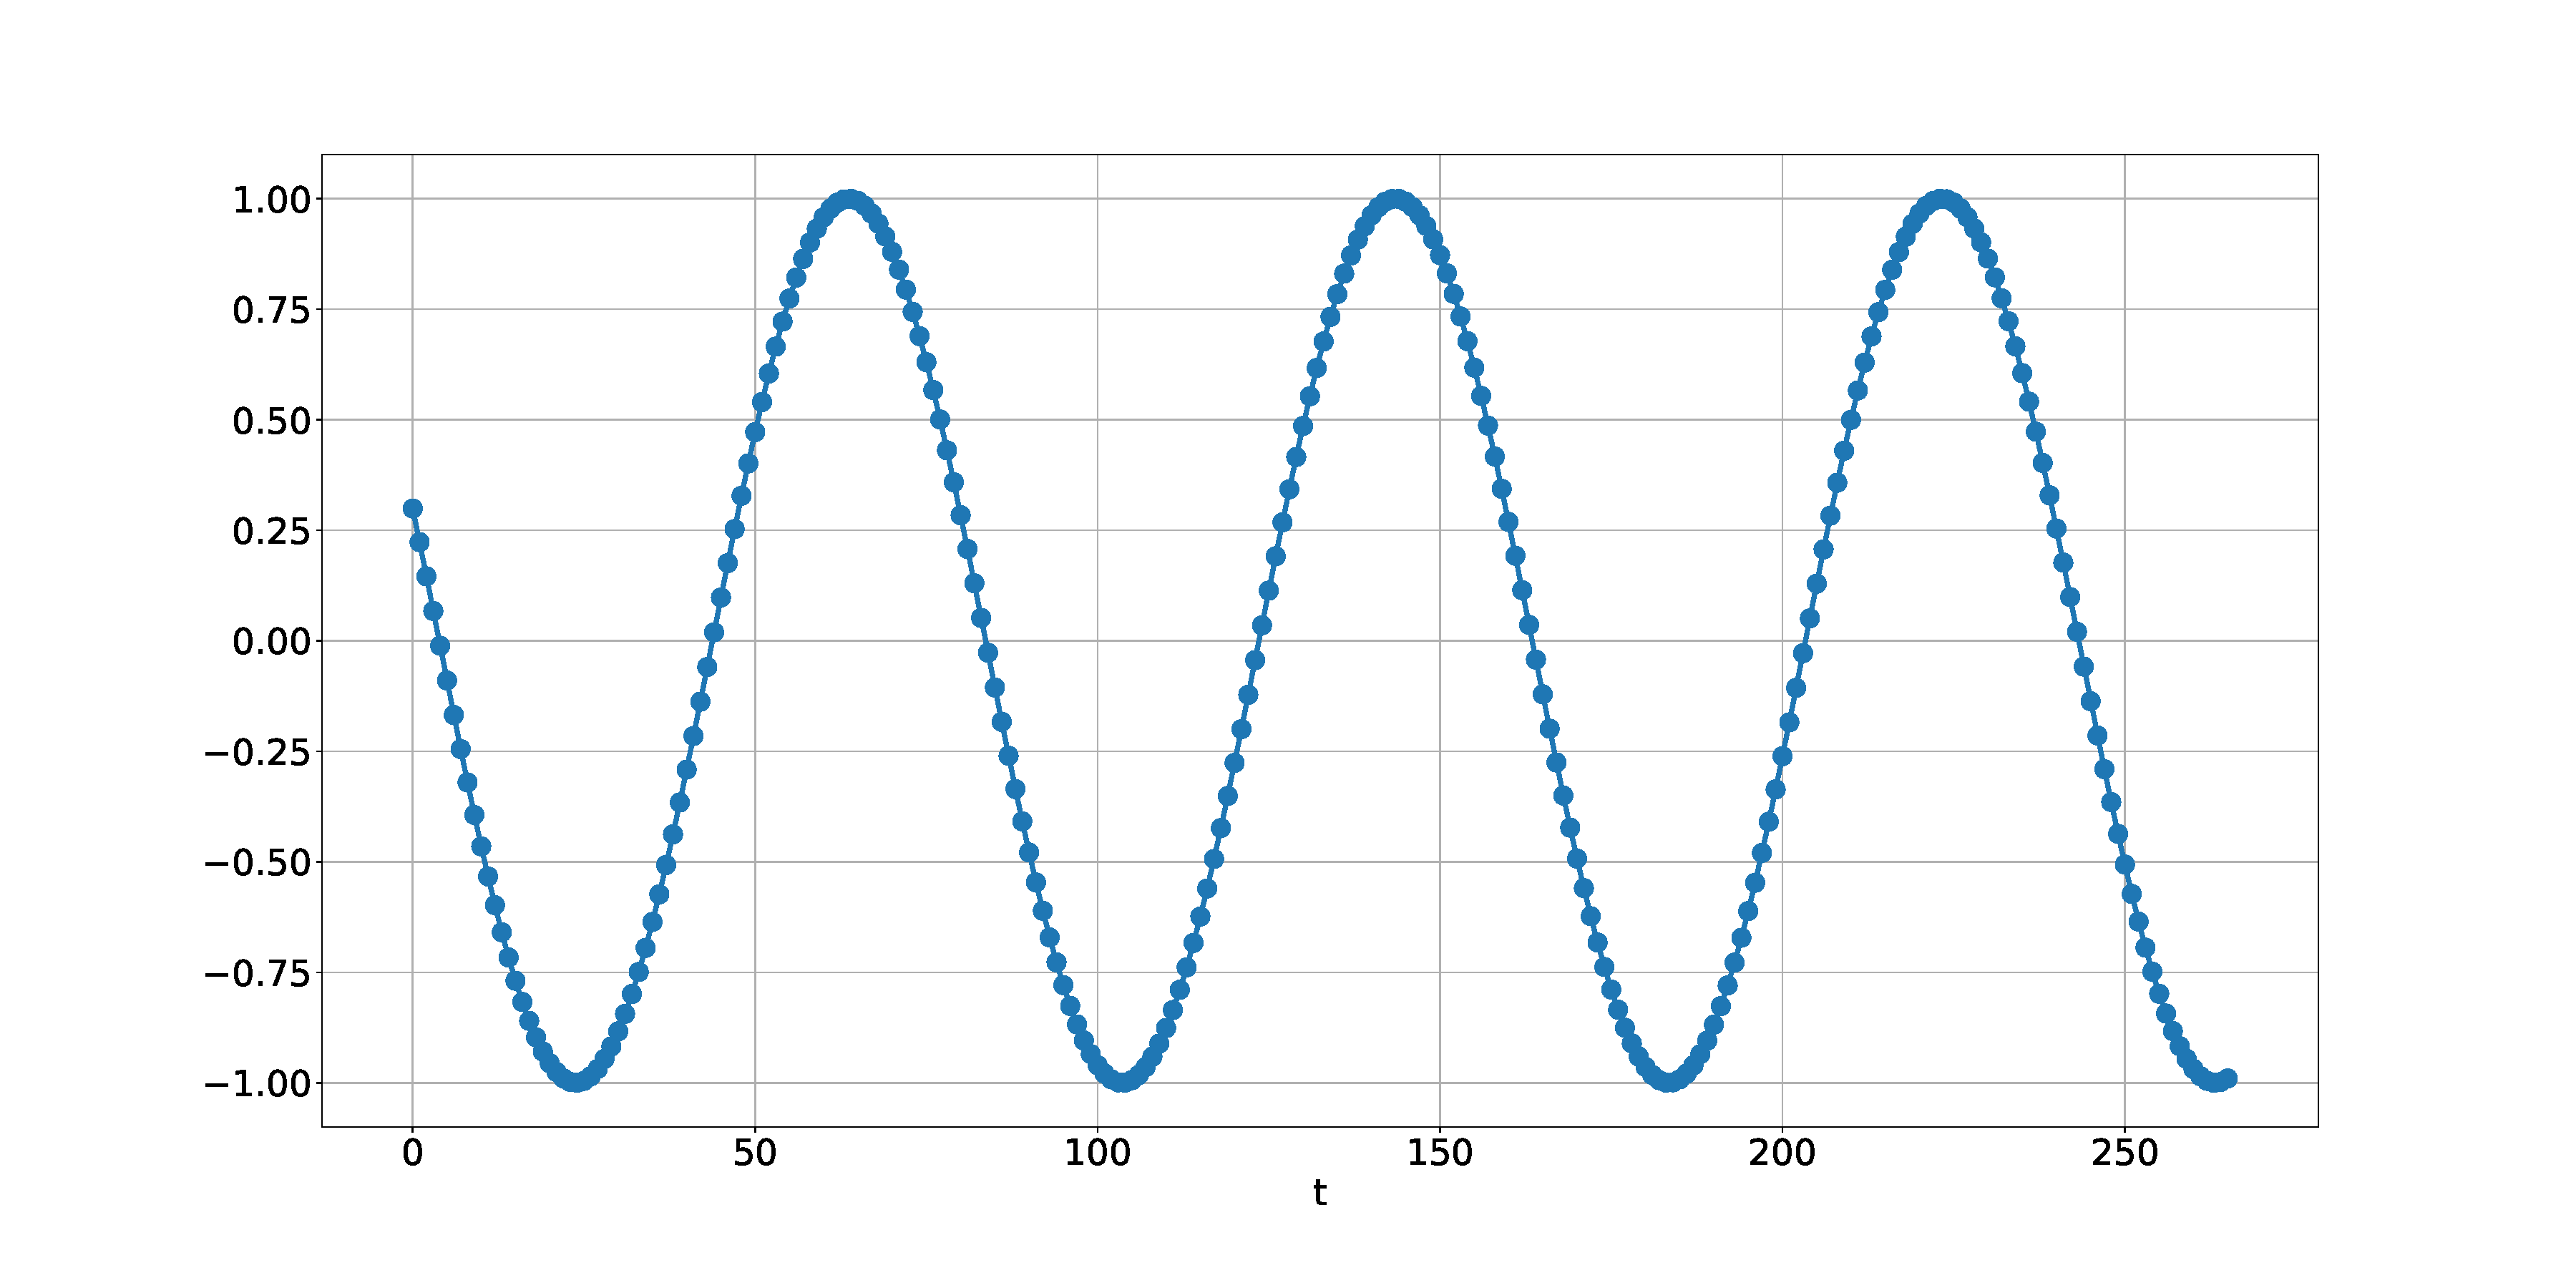
\includegraphics[width=0.5\textwidth]{figures/TimeSeries2_2dim.pdf}}\\
\subfloat[]{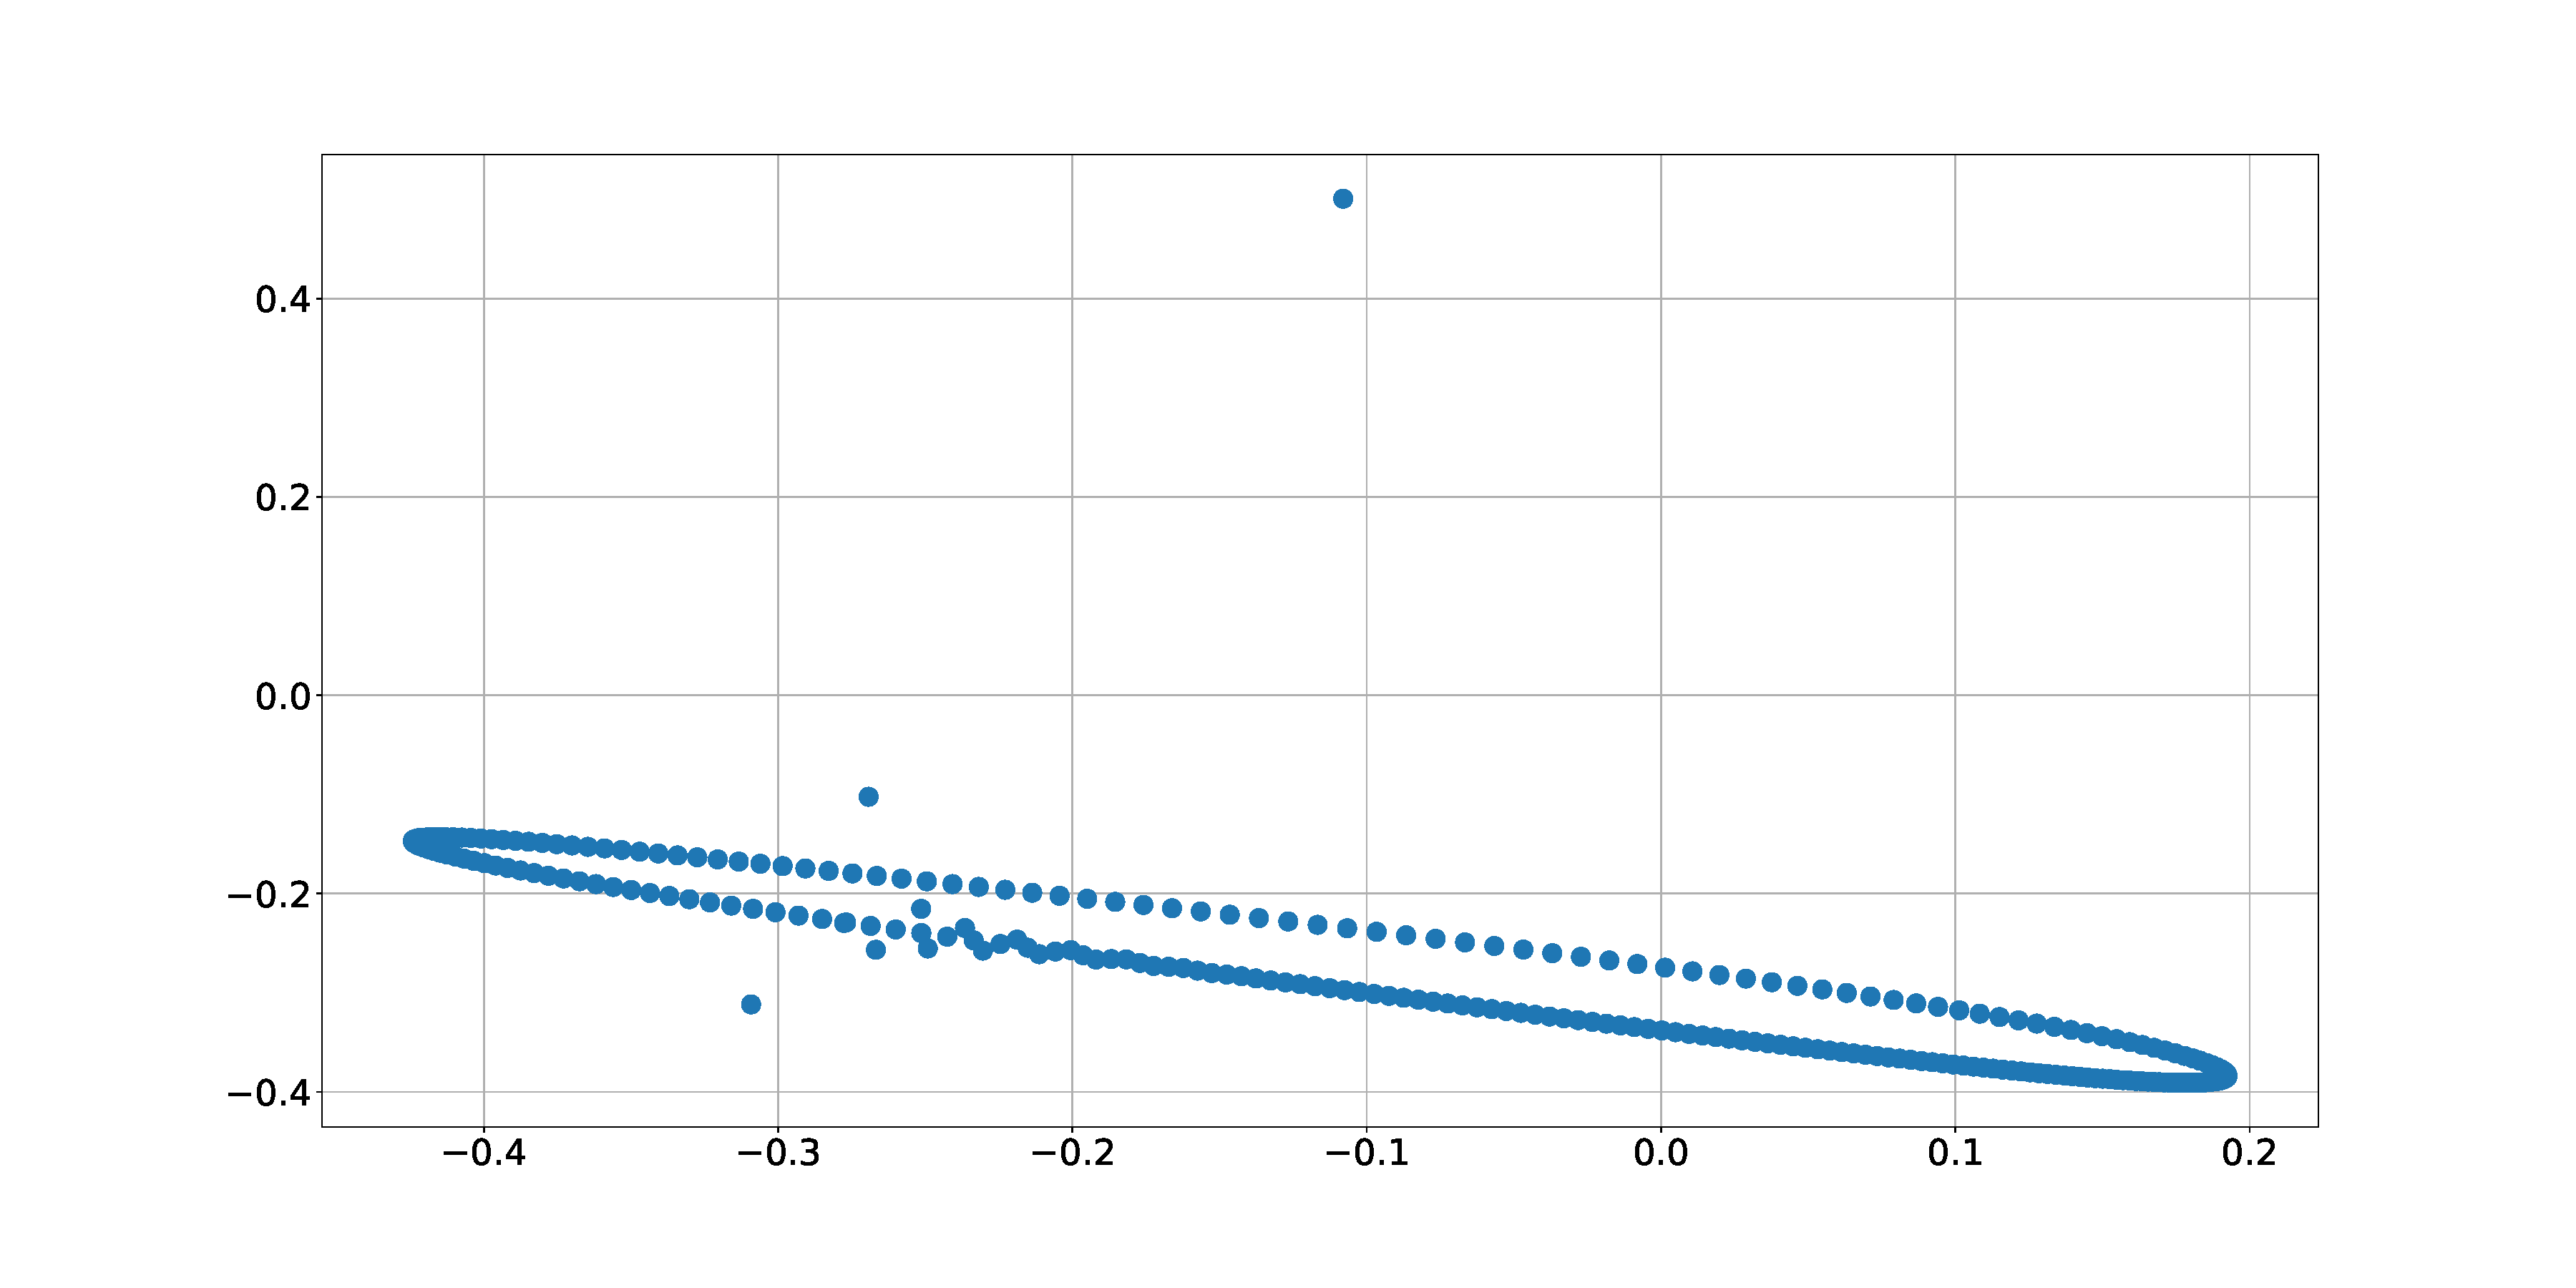
\includegraphics[width=0.5\textwidth]{figures/hidden1_2dim.pdf}}
\subfloat[]{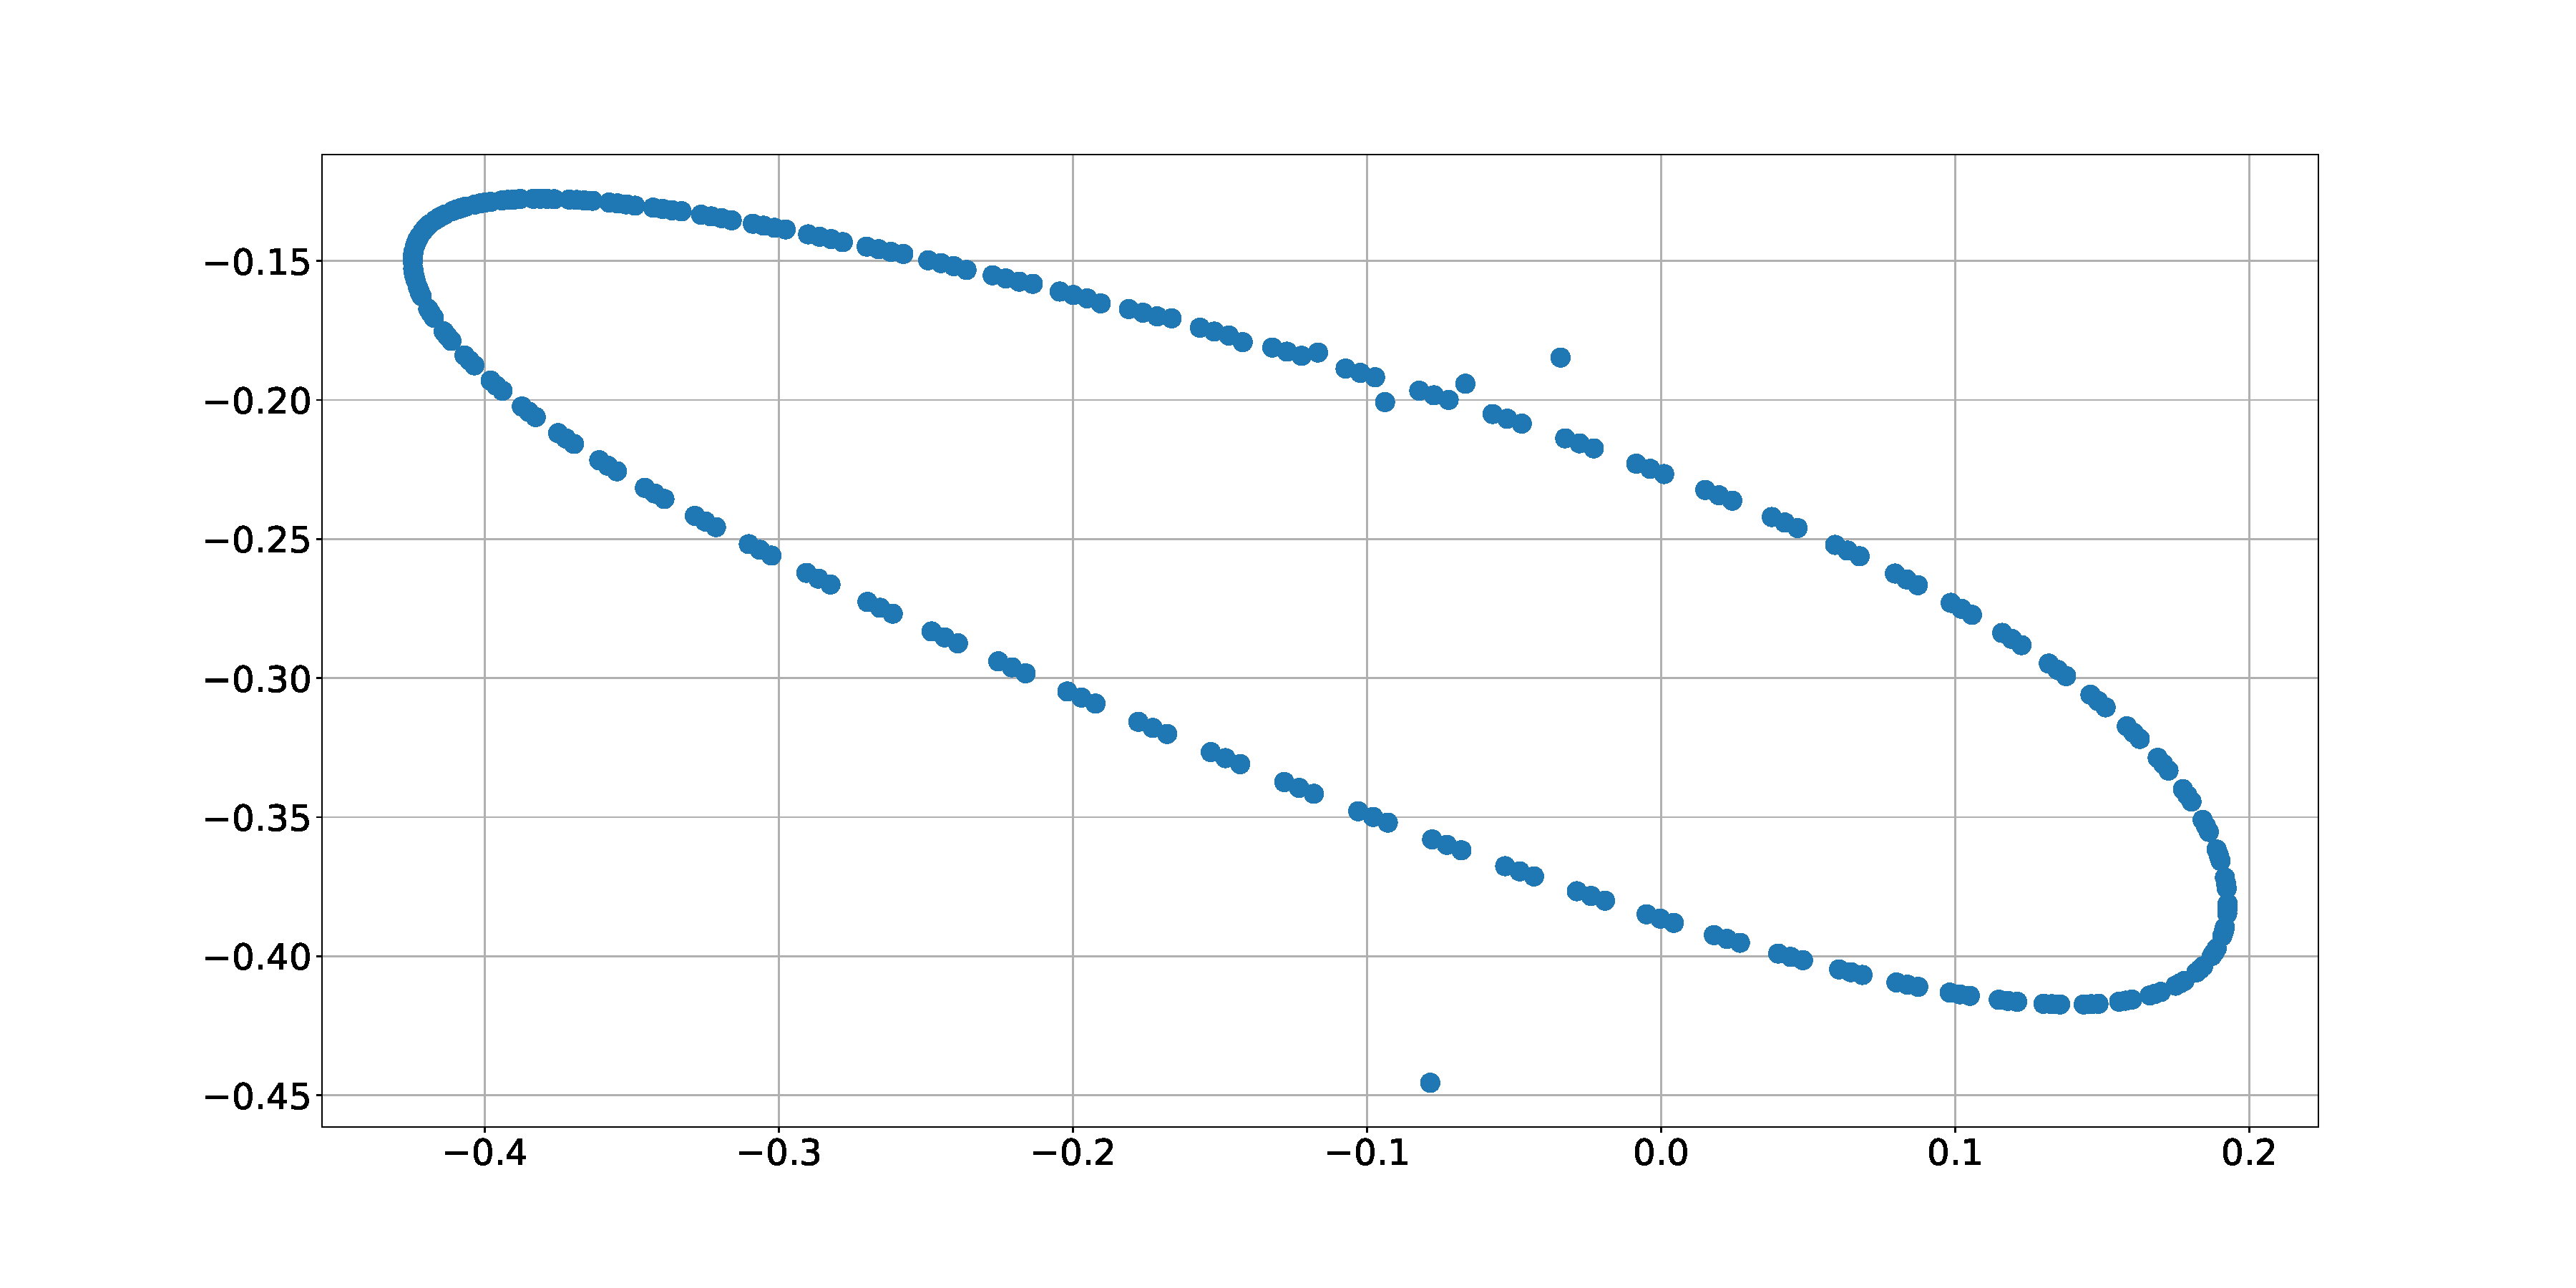
\includegraphics[width=0.5\textwidth]{figures/hidden2_2dim.pdf}}\\
\subfloat[]{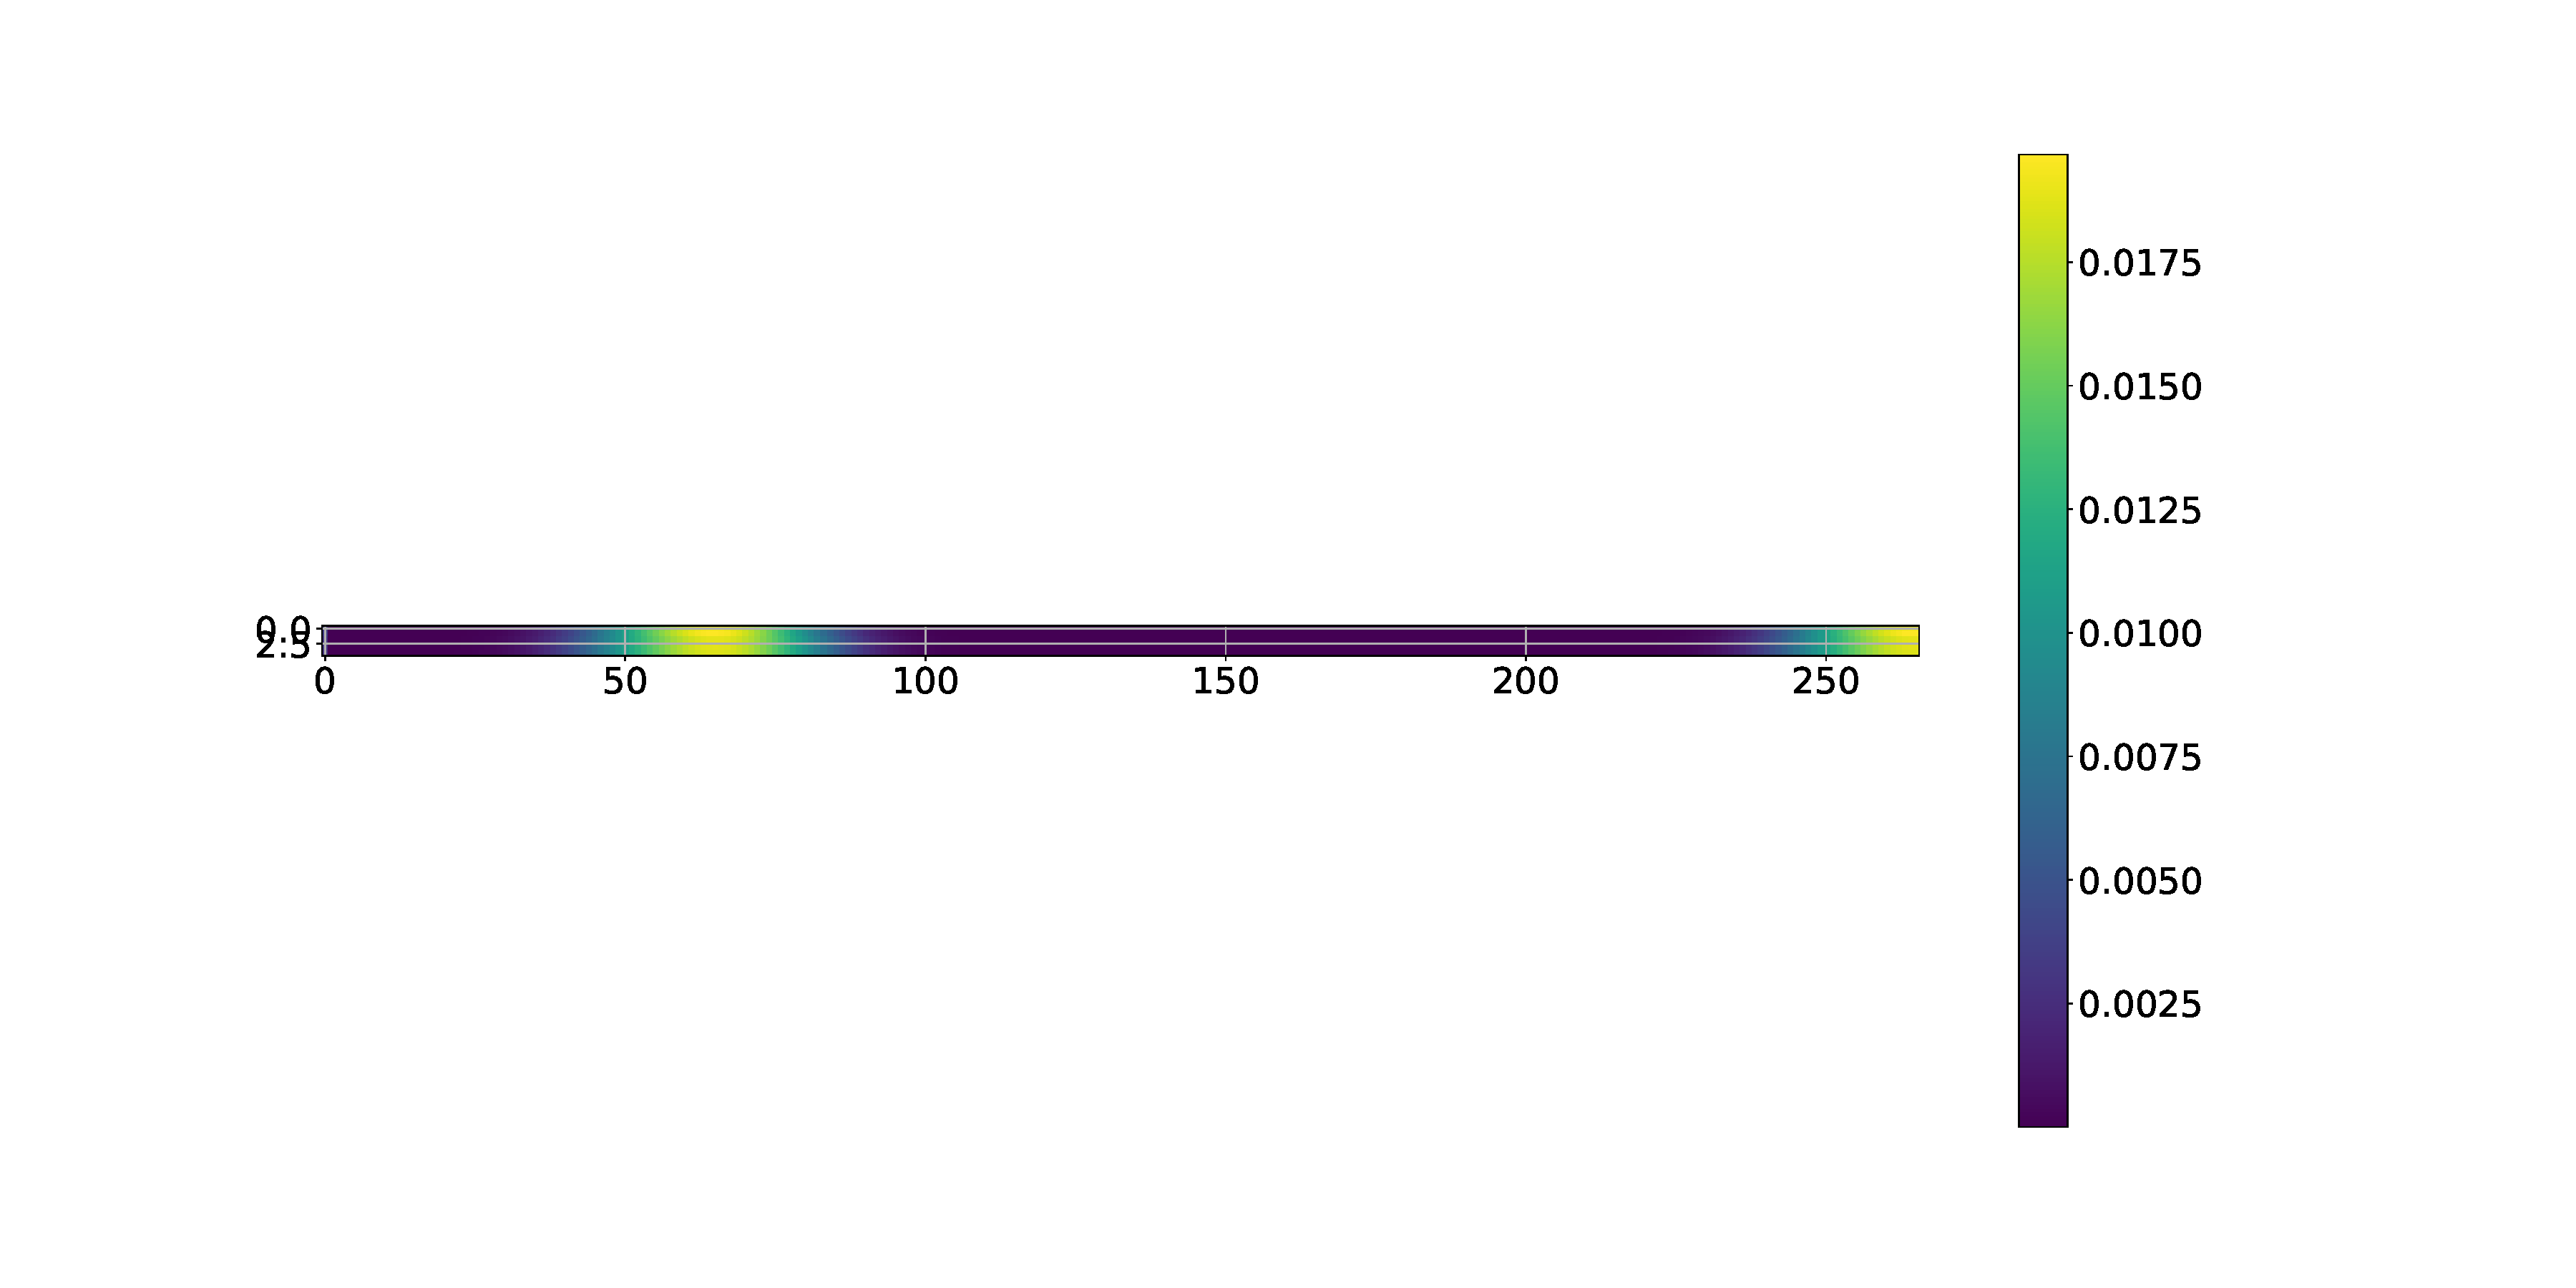
\includegraphics[width=0.5\textwidth]{figures/Attention1_2dim.pdf}}
\subfloat[]{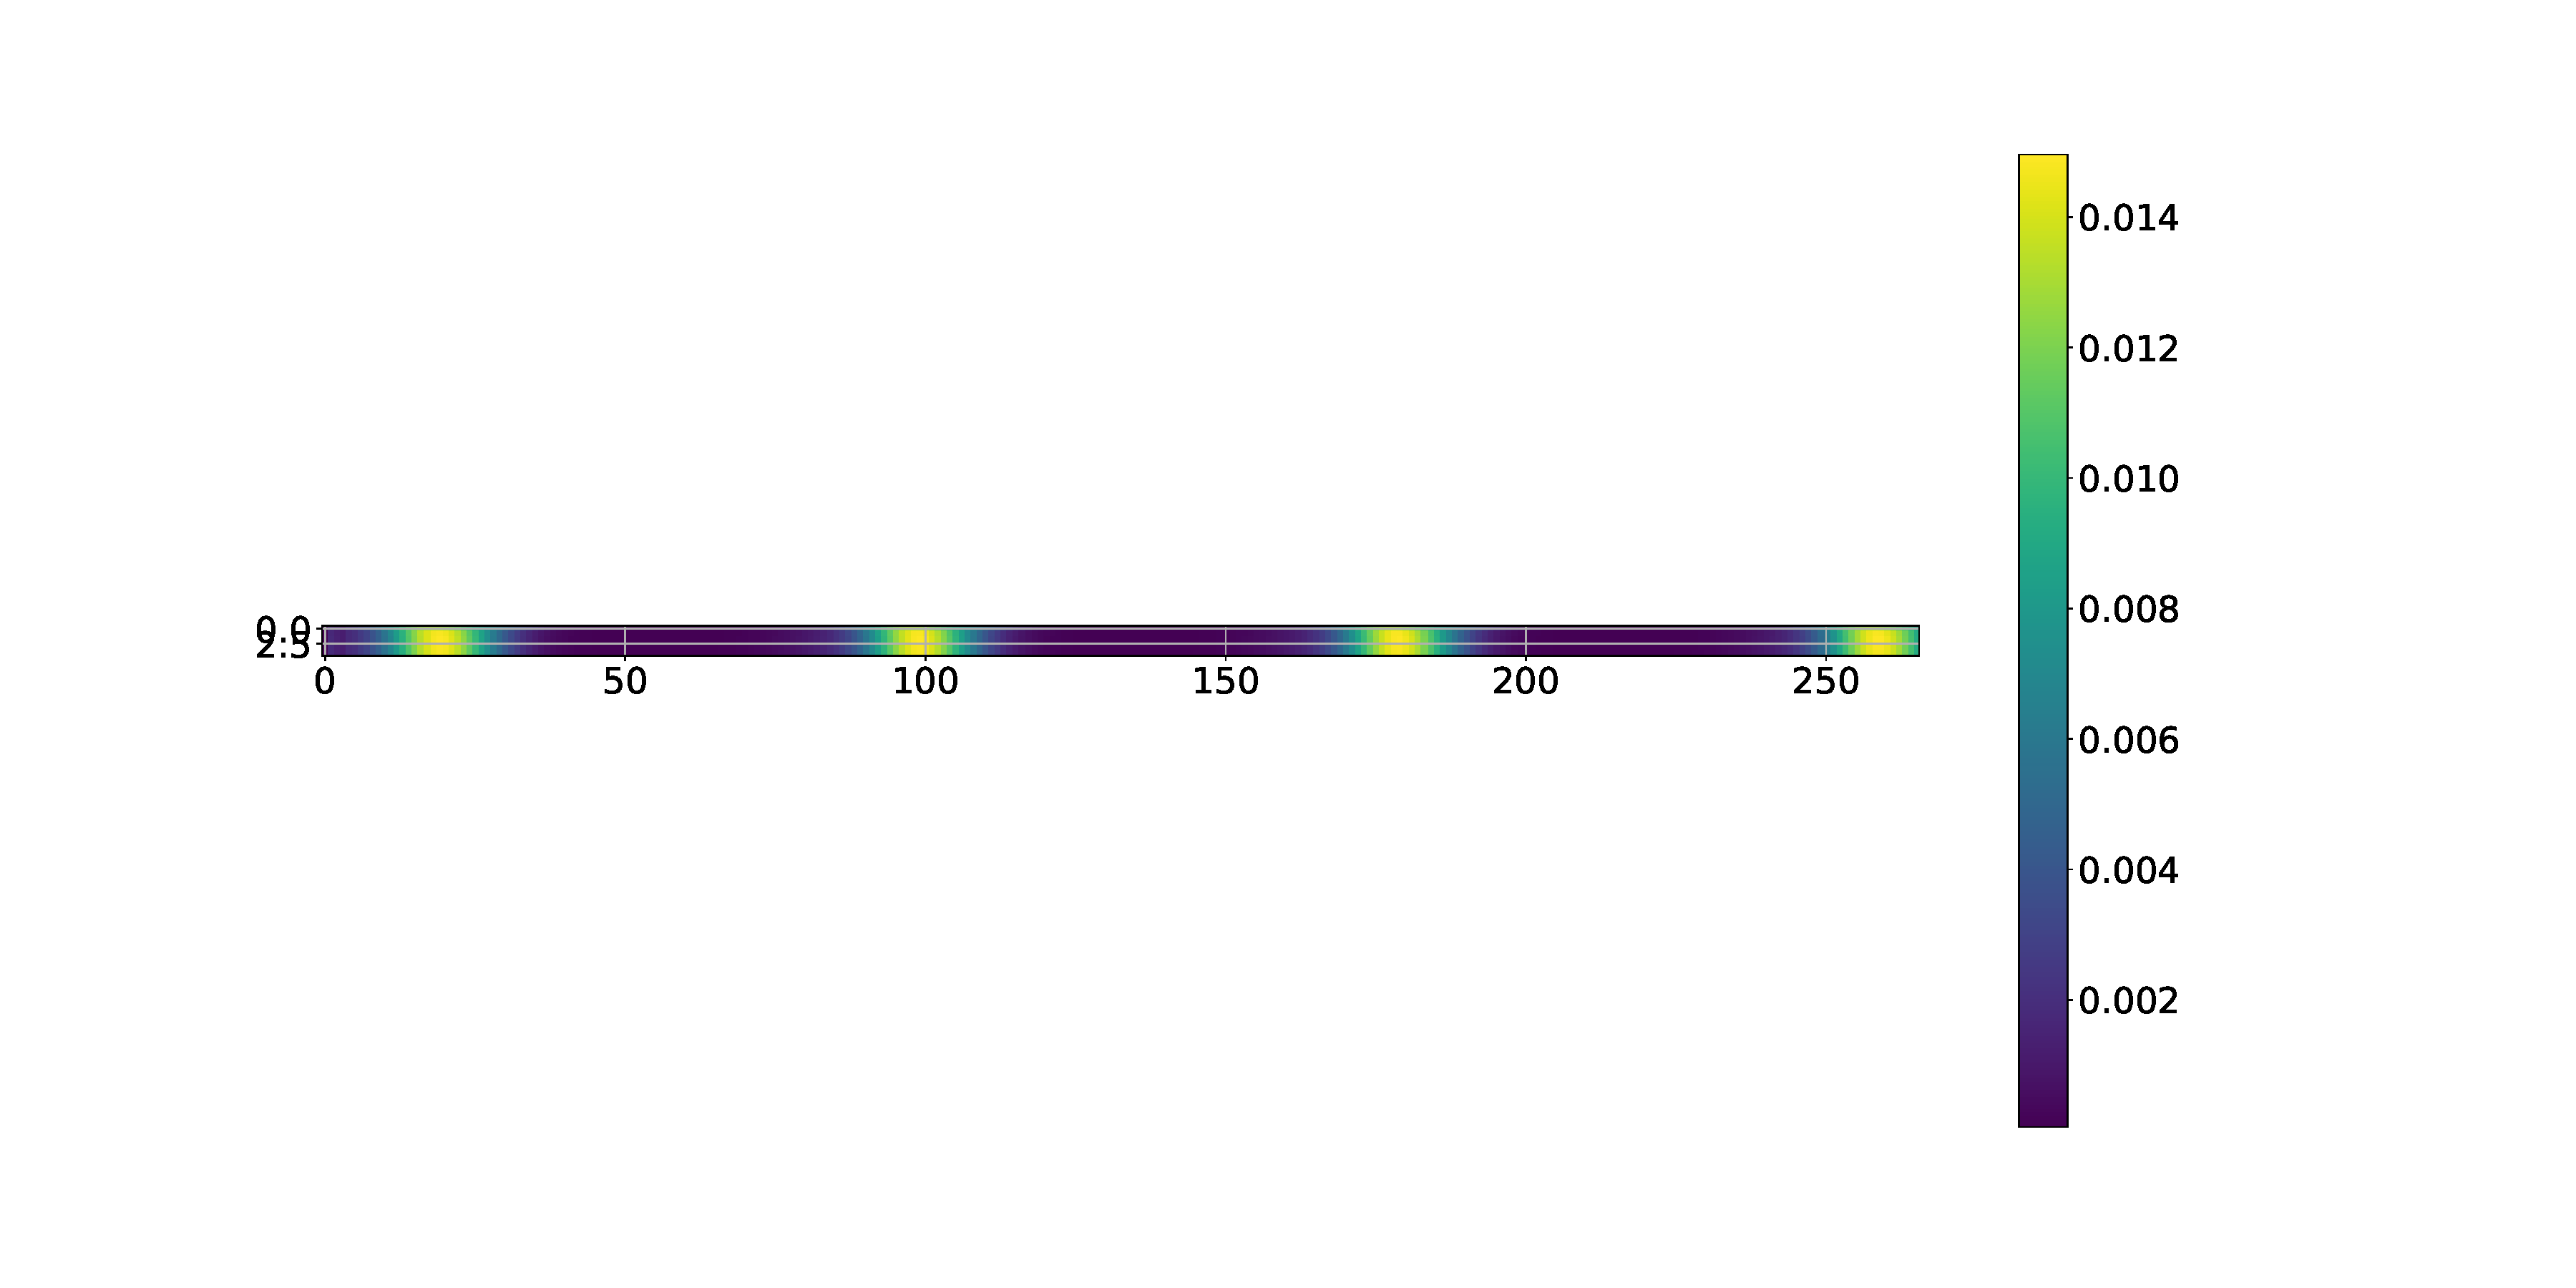
\includegraphics[width=0.5\textwidth]{figures/Attention2_2dim.pdf}}\\

\caption{Результаты для модели с рис.~\ref{fig1}}
\label{fig4}
\end{figure}

На рис.~\ref{fig4} показано, как для разных синусов выглядит скрытое пространство ecnoder'а, а также матрица Attention для генерации двух последующих точек в ряде.


\subsection{Эксперимент с простыми двумя простыми периодическими структурами внутри одного ряда}

Задача состоит в том, чтобы при помощи механизма Attention с временного ряда, который состоит из двух переодических сигналов (к примеру человек по очереди идет некоторое время и бежит некоторое время) выделить моменты времени где наблюдается первое действие и выделить моменты времени где наблюдается второе действие. 

Предлагается использовать seq2seq модель с Attention. 

Сама структура LSTM строит по сути фазовое пространство большой размерности. Попробуем обучить seq2seq модель, которая на вход принимает сигнал, который состоит из двух периодических сигналов, выдать на выход два сигнала, первый сигнал это чистый первый периодический сигнал со входа, а второй сигнал это второй периодический сигнал со входа. Тоесть другими словами, попробуем, сделать так, чтобы LSTM смогла из фазовому пространству вычленить два разных периодических сигнала. Для определенности будем считать первым периодическим сигналом тот сигнал который во временном ряде встретился раньше.

Как сделать чтобы LSTM по одному входу дала два сигнала???? У этого вопроса есть два возможных ответа:
\begin{itemize}
    \item первый случай простой, а давайте выход декодера будет не число а два числа --- значения первого сигнала и второго сигнала в один тик времени (простыми словами у нас есть 2 линейные модели которые по фазовому пространству делают некоторый предикт сигнала)
    
    \item второе решение немного сложнее (сейчас пробую сделать его). У нас есть как и раньше один выход LSTM. Но мы можем варьировать начальную точку LSTM с которой она начинает генерировать ряд. К примеру если мы хочем получить первый сигнал, что в качестве начальной точки дадим $0$ а если хочем сгенериить второй сигнал, то начальной точкой LSTM дадим $1$.
\end{itemize}
Ничего не получилось.
	
\begin{thebibliography}{99}
	\bibitem{cinar2018}
	\textit{Y. G. Cinar and H. Mirisaee} Period-aware content attention RNNs for time series forecasting with missing values~// Neurocomputing, 2018. Vol. 312. P. 177--186.
	
\end{thebibliography}
	

\end{document}

